\documentclass[10pt,a4paper]{article}
\usepackage{fontspec,amsmath,amssymb,amsthm,mathtools,graphicx,bm,bbm,stmaryrd,nicefrac}
\usepackage[margin=22mm]{geometry}
\usepackage[bookmarks=false]{hyperref}
\setlength{\emergencystretch}{3em}
\title{Prime-modulus quantum constant-depth circuits capture fanout}
\author{Daniel Grier, Jackson Morris}
\date{doi:10.4230/LIPIcs.CCC.2025.3; CC BY 4.0}
\begin{document}
\maketitle
\noindent\textit{Editorial note.} Editable TeX converted from the official CC BY HTML prose and math alttext. Original official PDF/HTML retained. Only the specified claim counts; all author context and available source-local supporting proofs are included.\par\medskip


\par\medskip\noindent\textbf{
1 Introduction}\par




To what extent are large multi-qubit gates useful for quantum computation? On the one hand, it is well-known that every multi-qubit gate can be decomposed into a circuit of simpler $1$- and $2$-qubit gates. On the other hand, this decomposition may introduce large overheads both in terms of gate count and circuit depth. Given that some multi-qubit gates might be experimentally feasible [22, 14, 16], it’s natural to ask what kinds of computational powers they unlock.\par




Specifically, we focus on the power of these large multi-qubit gates in constant depth. Such shallow circuits are experimentally appealing due to the possibility for less decoherence. Moreover, even shallow quantum circuits with $1$- and $2$-qubit gates are known to be surprisingly powerful, exhibiting quantum advantage in a variety of settings [4, 9, 25, 11]. Given the inherent complexity of simulating such circuits, there is the exciting possibility that augmenting these circuit models with large multi-qubit gates might lead to constant-depth implementations of practical quantum algorithms.\par




Much of the excitement about such circuit models is driven by a single gate – the multi-qubit Fanout gate – which is the quantum operation that copies \emph{classical} information:\par


\[\begin{gathered}
\mathsf{F}_{n}\left|b,x_{1},\ldots,x_{n}\right\rangle:=\left|b,x_{1}\oplus b,\ldots,x_{n}\oplus b\right\rangle
\end{gathered}\]


for all $b,x_{1},\ldots,x_{n}\in\{0,1\}$.\par




This seemingly innocuous gate (the classical analogue of which is included for free in almost every classical circuit model) turns out to be quite powerful. For starters, it is locally equivalent via conjugation by Hadamard gates to the quantum Parity gate [17],\par


\[\begin{gathered}
\mathsf{P}_{n}\left|b,x_{1},\ldots,x_{n}\right\rangle:=\left|b\oplus(x_{1}\oplus\cdots\oplus x_{n}),x_{1},\ldots,x_{n}\right\rangle,
\end{gathered}\]


which is a duality that has no classical counterpart [1]. Moreover, there are constant-depth quantum circuits with Fanout (and arbitrary single-qubit gates) for a wide variety of other symmetric Boolean operations such as And/Or and Majority [13, 24]. Perhaps most impressively, constant-depth quantum circuits with Fanout gates can factor integers with polynomial-time classical post-processing [13].\par




Given the centrality of Fanout to the story of low-depth circuits with multi-qubit gates, there has been significant work in trying to understand if other multi-qubit gates are similarly powerful. Most notably, it is widely believed that the multi-qubit generalization of the Toffoli gate is fundamentally less powerful than the Fanout gate in constant depth, and there is long line of work giving evidence that these generalized Toffoli gates cannot compute Fanout [3, 6, 21, 19, 18, 2]. In some sense, all of these results are grappling with a fundamental tension in the study of these low-depth circuit models – the high entanglement in the states produced by these circuits is an obstacle to proving lower bounds, but it is simultaneously unclear how one could leverage this complexity to implement a useful quantum algorithm.\par




There is a surprising dearth of low-depth circuit models with multi-qubit gates that are as powerful as Fanout. One natural\footnote{This candidate looks considerably more natural after considering the analogous landscape of \emph{classical} circuits, which we discuss in Section 1.1.} candidate for a gate that could be as powerful as Fanout is the quantum Threshold gate, a multi-qubit gate parameterized by some value $k\in\mathbb{N}$:\par


\[\begin{gathered}
\mathsf{Th}_{n,k}\left|b,x_{1},\ldots,x_{n}\right\rangle:=\left|b\oplus\mathbb{I}_{|x|\geq k},x_{1},\ldots,x_{n}\right\rangle
\end{gathered}\]


where $\mathbb{I}_{|x|\geq k}$ indicates if the Hamming weight of the input bit string $x=x_{1}\cdots x_{n}\in\{0,1\}^{n}$ is at least the target value $k$. In fact, Høyer and Špalek asked almost 20 years ago about the power of Threshold in constant depth [13]: “Can we simulate unbounded fan-out in constant depth using unbounded fan-in gates, e.g. $\operatorname{threshold}[t]$ or $\operatorname{exact}[t]$?” This question was reiterated more pointedly by Takahashi and Tani in 2011 [24]: “Does there exist a fundamental gate that is as powerful as an unbounded fan-out gate?”\par




We directly answer both of these questions in the affirmative by giving explicit constructions for Fanout using quantum Threshold gates:\par



% SOURCE-ID Thmtheorem1


\par\medskip\noindent\textbf{
\textbf{Theorem 1}\textbf{.}
}\par



\emph{There are poly-size constant-depth quantum circuits consisting of Threshold gates and arbitrary single-qubit gates that compute Fanout with high fidelity. Formally, ${\mathsf{BQTC}}^{0}={\mathsf{BQNC}}^{0}_{wf}$.}\par



% END-SOURCE-ID Thmtheorem1



The construction from this theorem actually reveals a number of other gates that are as fundamentally powerful as the Fanout gate. As it turns out, the salient feature of Threshold for our purposes is that it can be used to construct a sort of “weak” Parity gate – a gate that only acts non-trivially on inputs of the same parity.\par




Based on this idea, we introduce a class of multi-qubit phase gates that exhibit a generalization of this behavior. Formally, these gates are defined with respect to a set $S\subset\{0,1\}^{n}$ in the following way:\par


\[\begin{gathered}
U_{S}\left|x_{1},\ldots,x_{n}\right\rangle:=(-1)^{\mathbb{I}_{x\in S}}\left|x_{1},\ldots,x_{n}\right\rangle.
\end{gathered}\]


Crucially, we restrict our attention to “parity-restricted” sets $S$, that is, sets where all elements have the same parity (i.e., $x,y\in S\implies|x|\equiv|y|\pmod{2}$). We show that these weak parity gates can be bootstrapped in constant depth into true Parity gates (which, recall, are locally-equivalent to Fanout) albeit with the help of a few generalized Toffoli gates:\par



% SOURCE-ID Thmtheorem2


\par\medskip\noindent\textbf{
\textbf{Theorem 2}\textbf{.}
}\par



\emph{Let $\{S_{n}\}_{n}$ be a family of parity-restricted sets with size $|S_{n}|=\Theta(2^{n}/{\mathsf{poly}}(n))$. There are poly-size constant-depth quantum circuits consisting of $U_{S_{n}}$ gates, generalized Toffoli gates, and arbitrary single-qubit gates that compute Fanout with high fidelity.}\par



% END-SOURCE-ID Thmtheorem2



Since it is widely believed that multi-qubit Toffoli gates are not themselves sufficient to implement Fanout, the power of this construction likely derives from the weak parity gates. In fact, the reason these Toffoli gates were not required for Theorem 1 is due to the fact that Threshold can directly simulate Toffoli. In that vein, we also give conditions under which the $U_{S_{n}}$ gates alone suffice to simulate Parity; namely, when $|S_{n}|\geq 2^{n-O(1)}$ or $|S_{n}|\leq 2^{(1-\epsilon)n}$. Though, the latter condition will result in circuits of super-polynomial size.\par




While it has long been thought that Fanout/Parity gates were morally equivalent to other quantum modular arithmetic gates, those constructions seem to \emph{also} require these generalized Toffoli gates [8]. By a careful inspection of the original construction presented in [8] we find that generalized Toffoli gates are in fact not necessary. Formally, the quantum Mod-$p$ gates are defined as\par


\[\begin{gathered}
\mathsf{MOD}_{n,p}\left|b,x_{1},\ldots,x_{n}\right\rangle:=\left|b\oplus{\mathsf{Mod}}_{n,p}(x),x_{1},\ldots,x_{n}\right\rangle,
\end{gathered}\]


where ${\mathsf{Mod}}_{n,p}(x)$ is $1$ when $p$ divides the Hamming weight of $x=x_{1},\cdots,x_{n}\in\{0,1\}^{n}$. For example, the Mod-$2$ gate is essentially the Parity gate (up to a single-qubit $X$ gate). It is implicit in [8] that Fanout can be computed by a circuit consisting of Mod-$p$ gates and one- and two-qubit gates, yielding ${\mathsf{QNC}}^{0}_{wf}={\mathsf{QNC}}^{0}[2]\subseteq{\mathsf{QNC}}^{0}[q]$ for all $q\geq 2$, but not necessarily that ${\mathsf{QNC}}^{0}[p]={\mathsf{QNC}}^{0}[q]$ for distinct $p$ and $q$. The result they make explicit is that when Toffoli gates are allowed, any Mod-$q$ gate can be obtained using any other Mod-$p$ gate (by first implementing Fanout with Mod-$q$ gates and then computing Mod-$p$ with Fanout and generalized Toffoli gates). Concretely; ${\mathsf{QAC}}^{0}[p]={\mathsf{QAC}}^{0}[q]$ for $p,q\geq 2$. Only later was it shown that generalized Toffoli gates can be implemented using Fanout and single- and two-qubit gates, i.e., that ${\mathsf{QNC}}^{0}_{wf}={\mathsf{QAC}}^{0}_{wf}$ [13, 24]. In light of these results we observe the following:\par



% SOURCE-ID Thmtheorem3


\par\medskip\noindent\textbf{
\textbf{Theorem 3}\textbf{.}
}\par



\emph{For all $p,q\geq 2$, there are poly-size constant-depth quantum circuits consisting of Mod-$p$ gates and single-qubit gates that compute the Mod-$q$ operation. Formally, ${\mathsf{QNC}}^{0}[p]={\mathsf{QNC}}^{0}[q]$.}\par



% END-SOURCE-ID Thmtheorem3



\par\medskip\noindent\textbf{
1.1 Comparison to the classical setting}\par




Our focus on shallow circuits draws considerable inspiration from the analogous study of classical constant-depth circuit classes with large fan-in gates, which has been hugely influential in classical complexity theory. For instance, initial work in Boolean circuits saw the development of techniques for proving unconditional lower bounds such as random restrictions [1, 7, 27, 12], Fourier analytic methods [15], and polynomial methods [20, 23].\par




So how do we compare the quantum and classical settings? And what does this comparison tell us about the power of quantum circuits in constant depth? To start, classical circuits classes (e.g., ${\mathsf{NC}}^{0}$, ${\mathsf{AC}}^{0}$, ${\mathsf{TC}}^{0}$, …) typically assume that the output of any gate can be used as input for any number of other gates (i.e., a gate’s output can be “fanned out” to other gates). Of course, this is exactly the kind of fanout that immediately becomes so powerful when given to a constant-depth quantum circuit.\par




In fact, because of this fanout, the classical Threshold gate reigns supreme amongst similar classical circuit complexity classes. This is due to the fact that constant-depth classical circuits with Fanout and Threshold can compute any Boolean function where the output depends only on the Hamming weight of the input.\footnote{To see this, first notice that for any $k$, there is a constant-depth circuit with two Threshold gates that computes whether or not the input has Hamming weight exactly $k$. Since any symmetric Boolean function can be expressed as a disjunction over these “exact-$k$” clauses, the claim immediately follows due to the fact that a threshold of $1$ is equivalent to the Or function.} Formally, the complexity class ${\mathsf{TC}}^{0}$, which contains all languages computed by constant-depth classical circuits with Threshold, contains all other similarly defined classical circuit classes with other large fan-in gates: ${\mathsf{NC}}^{0}[p]$, ${\mathsf{AC}}^{0}$, ${\mathsf{AC}}^{0}[p]$, and ${\mathsf{ACC}}$.\footnote{See Definition 14 for precise definitions.} In many cases, Threshold is provably more powerful, e.g., ${\mathsf{AC}}^{0}\subsetneq{\mathsf{TC}}^{0}$ [1, 7] and ${\mathsf{AC}}^{0}[p]\subsetneq{\mathsf{TC}}^{0}$ [20, 23].\par




This is why the Threshold gate was a tantalizing target for quantum exploration. Prior to our work, it was \emph{not} known whether the quantum version of ${\mathsf{TC}}^{0}$ – i.e., ${\mathsf{BQTC}}^{0}$ – was as powerful as the quantum versions of the other classical complexity classes. In fact, given the surprising power of Fanout in the quantum world, the exact opposite was known: ${\mathsf{BQNC}}^{0}_{wf}\supseteq{\mathsf{BQTC}}^{0}$ [13]. That is, constant-depth quantum circuits with Fanout could simulate constant-depth circuits with Threshold. Our work restores order to the usually classical hierarchy, placing Threshold alongside Fanout as one of the most powerful quantum gates in constant depth: ${\mathsf{BQTC}}^{0}={\mathsf{BQNC}}^{0}_{wf}$.\par





\par\medskip\noindent\textbf{
1.2 Proof techniques and overview}\par




The constructions in Theorem 1 and Theorem 2 follow a general outline pioneered by Rosenthal [21]. There, it is shown that constant-depth quantum circuits can compute Fanout using generalized Toffoli gates \emph{provided exponential-sized circuits are allowed.} While not phrased in this language, Rosenthal’s construction shows a proof-of-principle technique for taking a very “weak” Parity gate (indeed, Toffoli non-trivially computes Parity for exactly one input!) and boosting it to a full Parity gate. We show that when we start with a gate (like Threshold) which is closer to Parity, this construction can be altered to yield circuits of polynomial size.\par




The proof goes in two steps. First, define a certain cat-like state called a “nekomata” [21]:\par


\[\begin{gathered}
\frac{\left|0^{n}\right\rangle\otimes\left|\psi_{0}\right\rangle+\left|1^{n}\right\rangle\otimes\left|\psi_{1}\right\rangle}{\sqrt{2}}
\end{gathered}\]


where $\left|\psi_{0}\right\rangle$ and $\left|\psi_{1}\right\rangle$ are arbitrary states. Following a similar idea to that of Green et al.  [8], such states can be used to compute Parity in constant depth using the relative phase between the $\left|0^{n}\right\rangle$ and $\left|1^{n}\right\rangle$ part of the state.\par




Second, show there is an explicit constant-depth construction for a nekomata state. Here, we show the key ingredient is the ability to create a “noisy” version of a usual cat state, where the all-zeroes and all-ones outcomes have noticeably larger amplitudes than those on the other outcomes. Threshold gates are significantly better at this task than the Toffoli gates in Rosenthal’s original construction. Finally, these states can be combined together (using Toffoli or Threshold gates) to form a high-fidelity nekomata state, completing the construction.\par





\par\medskip\noindent\textbf{
1.3 Related work}\par




Our work shares some similarity to that of [10], where the authors explore quantum advantage with constant-depth quantum circuits. They also make a similar claim suggesting that ${\mathsf{QTC}}^{0}={\mathsf{QNC}}^{0}_{wf}$, but crucially, their results hold in a circuit model with intermediate measurements and classical fanout. The classical fanout in their circuit model allows them to bootstrap the poor man’s cat state construction of Bene Watts et al. [26] to construct an actual cat state, an idea that was also explored in [5]. To be clear, our circuit model and definition of ${\mathsf{BQTC}}^{0}$ follows in a traditional line of work (e.g, [17, 8, 13, 24, 19, 21, 18]), where no such intermediate measurements or classical fanout is allowed. Therefore, we must use entirely different techniques.\par





\par\medskip\noindent\textbf{
1.4 Future directions}\par




One immediate question left open by our work is whether the approximation error inherent in the construction used to prove Theorem 1 can be eliminated without incurring a size or depth blow-up.
More generally, we ask which other conditions on a family of multi-qubit gates lead to powerful shallow circuits. One explicit approach would be to ask what properties of the sets $S$ parameterizing our phase gates $U_{S}$ are sufficient to compute Fanout. Is there a sufficient condition beyond being parity restricted?\par




Another interesting question concerns the circuit complexity of restricted families of threshold functions. Specifically, consider the Exact-$k$ gate, which indicates if the Hamming weight of the input is exactly $k$. Notice that Exact-$k$ can be constructed from two Threshold gates. Moreover, for $k\approx n/2$, Exact-$k$ can be used to compute Threshold. This latter statement is not obvious and follows from the fact that our proof of Theorem 1 actually uses Exact gates rather than Threshold gates. Indeed, for any constant $\alpha>0$ and any $k\in[n^{\alpha},n-n^{\alpha}]$ the gates $\mathsf{EX}_{k/2}$, $\mathsf{Th}_{k}$ and $\mathsf{P}_{n}$ are all equivalent under ${\mathsf{QAC}}^{0}$ reductions (see Theorem 22). However, it is unclear if this remains true for $k$ which is sub-polynomial in $n$, say $k=\log{n}$.\par






\par\medskip\noindent\textbf{
2 Preliminaries}\par




We will now introduce the different types of entangling gates considered in this work, the types of circuits constructed from them, and the complexity classes to which they roughly correspond.\par




\par\medskip\noindent\textbf{
2.1 Multi-qubit Gates}\par




A simple multi-qubit gate is the $\mathsf{CNOT}$ gate which acts on two qubits, flipping the target conditioned on the control, i.e.,\par


\[\begin{gathered}
\displaystyle\mathsf{CNOT}\left|x_{1},x_{2}\right\rangle=\left|x_{1},x_{1}\oplus x_{2}\right\rangle
\end{gathered}\]


Any two-qubit gate can be constructed from constantly many single-qubit gates and $\mathsf{CNOT}$ gates. A circuit consisting entirely of arbitrary single- and two-qubit gates is said to be a ${\mathsf{QNC}}$ circuit.\par




Another multi-qubit gate of interest is the Toffoli gate, which acts on three qubits by flipping the last qubit controlled on the first two, i.e.,\par


\[\begin{gathered}
\displaystyle\text{Tof}\left|x,y,z\right\rangle=\left|x,y,(x\land y)\oplus z\right\rangle
\end{gathered}\]


This gate can be seen as a $\mathsf{CNOT}$ gate with an additional control qubit. In fact, we call the analogous unitary on $n>1$ qubits a \emph{generalized} Toffoli gate:\par



% SOURCE-ID Thmtheorem4


\par\medskip\noindent\textbf{
\textbf{Definition 4}\textbf{.}
}\par



\emph{The generalized Toffoli gate $\land_{n}$ acts on $n+1$ qubits by computing the $\mathsf{AND}$ of the first $n$ bits in superposition. For all $x_{1},x_{2},\dots x_{n},b\in\{0,1\}$ the $\wedge_{n}$-gate acts as}\par


\[\begin{gathered}
\displaystyle\land_{n}\left|x_{1},x_{2},\dots x_{n},b\right\rangle=\left|x_{1},x_{2},\dots x_{n},(x_{1}\land\cdots\land x_{n})\oplus b\right\rangle
\end{gathered}\]



% END-SOURCE-ID Thmtheorem4



Circuits composed of arbitrary single-qubit gates and generalized Toffoli gates are referred to as ${\mathsf{QAC}}$ circuits.\par



% SOURCE-ID Thmtheorem5


\par\medskip\noindent\textbf{
\textbf{Definition 5}\textbf{.}
}\par



\emph{For $k\in\{0,1\dots n\}$ and $x_{1},x_{2},\dots x_{n},b\in\{0,1\}$ the unitary $\mathsf{Th}_{n,k}$ acts as}\par


\[\begin{gathered}
\displaystyle\mathsf{Th}_{n,k}\left|b\right\rangle\left|x\right\rangle=\left|b\oplus\mathbb{I}_{|x|\geq k}\right\rangle\left|x\right\rangle
\end{gathered}\]



% END-SOURCE-ID Thmtheorem5



Circuits composed of arbitrary single-qubit gates and threshold gates\footnote{Recall that a function $f\colon\{0,1\}^{n}\to\{0,1\}$ is said to be a \emph{threshold function} if it can be written as





$\displaystyle f(x)=\begin{cases}1&\sum_{i=1}^{n}w_{i}x_{i}\geq b\\
0&\text{otherwise}\end{cases}$


for some $w_{1},\dots w_{n},b\in\mathbb{R}$. For our purposes it suffices to only consider threshold functions in which $w_{i}=1$ for all $i\in[n]$.} are said to be ${\mathsf{QTC}}$ circuits. Note that by taking $k=n$ we recover the generalized Toffoli gate, and in this sense the generalized Toffoli gate \emph{is} a Threshold gate, so including this gate in the allowed gate-set for ${\mathsf{QTC}}$ circuits would be redundant.\par




Note that in the above definition we allow for the use of any threshold gate in ${\mathsf{QTC}}$ circuits, but this is actually not necessary, even in constant depth. As we will later show, it suffices to have a usual threshold, $\mathsf{Th}_{n,k}$, or exact, $\mathsf{EX}_{n,k}$, gate with $k={\mathsf{poly}}(n)$ to recover the full computational power of ${\mathsf{QTC}}$ as is defined above. In other words, any sufficiently powerful $\mathsf{EX}_{n,k}$ or $\mathsf{Th}_{n,k}$ gate can be leveraged to recover \emph{all other} threshold and exact gates in constant-depth and polynomial-size. This reduction is non-trivial and combines our main result with the constant-depth constructions given in [13] for computing arbitrary threshold gates with fanout. A full explanation is given in Theorem 22.\par




Let $U_{f}$ be the unitary which computes some boolean function $f:\{0,1\}^{n}\to\{0,1\}$ in superposition, i.e., for all $x\in\{0,1\}^{n}$ and $b\in\{0,1\}$ $U_{f}\left|x,b\right\rangle=\left|x,b\oplus f(x)\right\rangle$. Note that all multi-qubit gates discussed thus far fall into this category. Now, observe that when the target qubit is replaced with $\left|-\right\rangle=\frac{\left|0\right\rangle-\left|1\right\rangle}{\sqrt{2}}$, we can “compute $f$ in the phase”:\par


\[\begin{gathered}
\displaystyle U_{f}\left|-\right\rangle\left|x\right\rangle=(-1)^{f(x)}\left|-\right\rangle\left|x\right\rangle
\end{gathered}\]


So, given $U_{f}$ we can with a single ancilla implement $V_{f}$ which acts as $V_{f}\left|x\right\rangle=(-1)^{f(x)}\left|x\right\rangle$. While going from $U_{f}$ to $V_{f}$ is not a difficult task the converse could in general be quite non-trivial.\footnote{For instance, take $Z^{\otimes n}$; this gate computes parity in the phase as $Z^{\otimes n}\left|x\right\rangle=(-1)^{|x|}\left|x\right\rangle$, but it is unclear if there is a simple way to recover the usual parity gate: $\mathsf{P}_{n}$.}\par




As mentioned, the \emph{quantum Fanout gate} gives us some way of “copying” a given qubit and $\mathsf{XOR}$-ing it onto an unbounded number of qubits.\par



% SOURCE-ID Thmtheorem6


\par\medskip\noindent\textbf{
\textbf{Definition 6}\textbf{.}
}\par



\emph{For all $x_{1},x_{2},\dots x_{n},b\in\{0,1\}$ the Fanout unitary, $\mathsf{F}_{n}$, acts as}\par


\[\begin{gathered}
\displaystyle\mathsf{F}_{n}\left|b\right\rangle\left|x_{1},x_{2},\dots x_{n}\right\rangle=\left|b\oplus x_{1},b\oplus x_{2},\dots b\oplus x_{n}\right\rangle
\end{gathered}\]



% END-SOURCE-ID Thmtheorem6



We will refer to circuits constructed from one- and two-qubit and Fanout gates as ${\mathsf{QNC}}_{wf}$ circuits.\par




Another important class of gates are so-called $\mathsf{MOD}$ gates:\par



% SOURCE-ID Thmtheorem7


\par\medskip\noindent\textbf{
\textbf{Definition 7}\textbf{.}
}\par



\emph{For a given $m\in\mathbb{N}$ and all $x_{1},x_{2},\dots x_{n},b\in\{0,1\}$ the $\mathsf{MOD}_{n,m}$ gate acts as}\par


\[\begin{gathered}
\displaystyle\mathsf{MOD}_{n,m}\left|x_{1},x_{2},\dots x_{n}\right\rangle\left|b\right\rangle=\left|x_{1},x_{2},\dots x_{n}\right\rangle\left|{\mathsf{Mod}}_{n,m}(x)\oplus b\right\rangle
\end{gathered}\]


\emph{Where ${\mathsf{Mod}}_{n,m}(x)=1$ iff $|x|$ is divisible by $m$. Further, for $\ell\in\{0,1,\dots m-1\}$ we use ${\mathsf{Mod}}_{n,m,\ell}(x)$ to denote the function which is $1$ iff $|x|\equiv\ell\;(\mathrm{mod}\;m)$ and the corresponding quantum gate accordingly:}\par


\[\begin{gathered}
\displaystyle\mathsf{MOD}_{n,m,\ell}\left|b\right\rangle\left|x_{1},x_{2},\dots x_{n}\right\rangle=\left|{\mathsf{Mod}}_{n,m,\ell}(x)\oplus b\right\rangle\left|x_{1},x_{2},\dots x_{n}\right\rangle.
\end{gathered}\]



% END-SOURCE-ID Thmtheorem7



Note that when $m=2$ the $\mathsf{MOD}_{n,2,1}$ gate is equivalent to the parity gate $\mathsf{P}_{n}$. When a circuit consists of one- and two-qubit gates and $\mathsf{MOD}_{n,m}$ gates for a fixed $m$ it is called a ${\mathsf{QNC}}[m]$ circuit and when the circuit also contains generalized Toffoli gates it is referred to as a ${\mathsf{QAC}}[m]$ circuit.\par




The final class of gates we will define are what we call “parity-restricted” gates which have not previously appeared in the literature. A set of bit strings $S\subseteq\{0,1\}^{n}$ is said to be \emph{parity restricted} if $|s_{1}|\equiv|s_{2}|\pmod{2}$ for all $s_{1},s_{2}\in S$.\par



% SOURCE-ID Thmtheorem8


\par\medskip\noindent\textbf{
\textbf{Definition 8}\textbf{.}
}\par



\emph{For a given set $S\subset\{0,1\}^{*}$ we define the $n$-qubit gate $U_{S,n}$ as}\par


\[\begin{gathered}
\displaystyle U_{S,n}\left|x\right\rangle=(-1)^{\mathbb{I}_{S}(x)}\left|x\right\rangle
\end{gathered}\]


\emph{Further, we call $U_{S,n}$ a parity-restricted gate if $|x|\equiv|y|\mod{2}$ for all $x,y\in S$.}\par



% END-SOURCE-ID Thmtheorem8



We will often drop the $n$ subscript from $U_{S,n}$ when discussing sets $S$ which only consist of strings of the same length, i.e. $S\subset\{0,1\}^{n}$ for some $n$.\par




For a given parity-restricted set $S$, a circuit consisting of arbitrary one- and two-qubit gates and $U_{S,n}$ gates for $n\in\mathbb{N}$ is said to be a ${\mathsf{QNC}}_{S}$ circuit. Similarly, if the circuit also consists of generalized Toffoli gates the circuit is said to be a ${\mathsf{QAC}}_{S}$ circuit. Indeed, the parity-restrict condition can be dropped, but in this work we will only consider $S$ which are parity-restricted sets.\par




Finally, we will define the primary complexity measures for quantum circuits.\par



% SOURCE-ID Thmtheorem9


\par\medskip\noindent\textbf{
\textbf{Definition 9}\textbf{.}
}\par



\emph{A quantum circuit $C$ is said to have depth $d$ if $C$ can be decomposed as a sequence $M_{d}S_{d}\cdots M_{2}S_{2}M_{1}S_{1}$ where each $S_{i}$ consists entirely of single-qubit gates and $M_{i}$ consists of non-overlapping multi-qubit gates (i.e., every pair of gates in $M_{i}$ operate on disjoint sets of qubits).}\par



% END-SOURCE-ID Thmtheorem9


% SOURCE-ID Thmtheorem10


\par\medskip\noindent\textbf{
\textbf{Definition 10}\textbf{.}
}\par



\emph{A quantum circuit $C$ has size $s$ if $C$ has exactly $s$ multi-qubit gates.}\par



% END-SOURCE-ID Thmtheorem10




\par\medskip\noindent\textbf{
2.2 Quantum Circuit Complexity Classes}\par




In this section we will define the relevant quantum circuit classes, but before doing that we must introduce the notion of a circuit family and what it means for a circuit family to compute a Boolean function.\par



% SOURCE-ID Thmtheorem11


\par\medskip\noindent\textbf{
\textbf{Definition 11}\textbf{.}
}\par



\emph{A family of quantum circuits is a collection $\mathcal{C}=\{C_{n}\}_{n\geq 1}$ where $C_{n}$ acts on $n+a(n)$ qubits where $a(n)$ is some computable function.}\par



% END-SOURCE-ID Thmtheorem11



This definition of a circuit family is analogous to the classical notion of a \emph{non-uniform} circuit family since there need not be any relation between circuits for different sizes (e.g., it is not necessary for there to exist a Turing machine which outputs a description of $C_{n}$ on input $1^{n}$. Such a requirement is only for \emph{uniform} circuit families). It should be noted that all constructions presented in this work correspond to uniform circuit families nonetheless.\par



% SOURCE-ID Thmtheorem12


\par\medskip\noindent\textbf{
\textbf{Definition 12}\textbf{.}
}\par



\emph{For a given language $L\subseteq\{0,1\}^{*}$ we say that a family of quantum circuits $\{C_{n}\}_{n\geq 1}$ each acting on $n+a(n)$ qubits exactly computes $L$ if for all $n\geq 1$ and $x\in\{0,1\}^{n}$ measuring the last qubit of $C_{n}\left|x\right\rangle\left|0^{a(n)}\right\rangle$ in the computational basis yields}\par


\begin{itemize}


\item[] 
$\blacksquare$ 


$\left|1\right\rangle$\emph{ with certainty if }$x\in L$\emph{}\par





\item[] 
$\blacksquare$ 


$\left|0\right\rangle$\emph{ with certainty if }$x\not\in L$\emph{}\par





\end{itemize}



% END-SOURCE-ID Thmtheorem12



Now, for the complexity classes of interest:\par


\begin{itemize}


\item[] 
$\blacksquare$ 


${\mathsf{QNC}}^{i}$ is the class of problems decidable by ${\mathsf{QNC}}$ circuits which act on polynomially-many qubits (i.e. $n+a(n)$ is bounded by some polynomial in $n$), have polynomial size and depth $O(\log^{i}(n))$.\par





\item[] 
$\blacksquare$ 


${\mathsf{QAC}}^{i}$ is the class of problems decidable by ${\mathsf{QAC}}$ circuits which act on polynomially-many qubits, have polynomial size and depth $O(\log^{i}(n))$.\par





\item[] 
$\blacksquare$ 


${\mathsf{QTC}}^{i}$ is the class of problems decidable by ${\mathsf{QTC}}$ circuits which act on polynomially-many qubits, have polynomial size and depth $O(\log^{i}(n))$.\par





\item[] 
$\blacksquare$ 


${\mathsf{QNC}}^{i}_{wf}$ is the class of problems decidable by ${\mathsf{QNC}}_{wf}$ circuits which act on polynomially-many qubits, have polynomial size and depth $O(\log^{i}(n))$.\par





\end{itemize}




The primary focus of this work will be constant depth circuits, which correspond to $i=0$ in the above definitions, i.e., the classes ${\mathsf{QNC}}^{0}$, ${\mathsf{QAC}}^{0}$, ${\mathsf{QTC}}^{0}$, and ${\mathsf{QNC}}_{wf}^{0}$.\par




Finally, we introduce two new complexity classes parameterized by sets $S\subset\{0,1\}^{*}$:\par


\begin{itemize}


\item[] 
$\blacksquare$ 


For a given set $S$, ${\mathsf{QNC}}_{S}^{i}$ is the class of problems decidable by ${\mathsf{QNC}}_{S}$ circuits which act on polynomially-many qubits, have polynomial size and depth $O(\log^{i}n)$.\par





\item[] 
$\blacksquare$ 


For a given set $S$, ${\mathsf{QAC}}_{S}^{i}$ is the class of problems decidable by ${\mathsf{QAC}}_{S}$ circuits which act on polynomially-many qubits, have polynomial size and depth $O(\log^{i}n)$.\par





\end{itemize}



% SOURCE-ID Thmtheorem13


\par\medskip\noindent\textbf{
\textbf{Proposition 13}\textbf{ }(Proposition 3.1 of [8])\textbf{.}
}\par



\emph{The following tasks are equivalent for constant-depth circuits consisting of $\wedge_{n}$-gates and single-qubit gates:}\par


\begin{enumerate}


\item[] 
1. 


\emph{Preparing the state }$\frac{\left|0^{n}\right\rangle+\left|1^{n}\right\rangle}{\sqrt{2}}$\emph{ from }$\left|0^{n}\right\rangle$\emph{ and performing the inverse transformation.}\par





\item[] 
2. 


\emph{Applying Fanout }$\mathsf{F}_{n}$\emph{.}\par





\item[] 
3. 


\emph{Applying Parity }$\mathsf{P}_{n}$\emph{.}\par





\end{enumerate}


\emph{In other words, these tasks are equivalent under ${\mathsf{QAC}}^{0}$ reductions.}\par



% END-SOURCE-ID Thmtheorem13



Critical to our construction is the fact that (1) in the above proposition can be relaxed to a more general state preparation task. To see how, we must define a class of a “cat-like” states, first introduced by Rosenthal [21] which he calls \emph{nekomata}:\par



% SOURCE-ID Thmtheorem14


\par\medskip\noindent\textbf{
\textbf{Definition 14}\textbf{.}
}\par



\emph{A state $\left|\phi\right\rangle$ on $n+m$ qubits is said to be an $n$-nekomata if there exists some ordering of the qubits such that}\par


\[\begin{gathered}
\displaystyle\left|\phi\right\rangle=\frac{\left|0^{n}\right\rangle\otimes\left|\psi_{0}\right\rangle+\left|1^{n}\right\rangle\otimes\left|\psi_{1}\right\rangle}{\sqrt{2}}
\end{gathered}\]


\emph{where $\left|\psi_{0}\right\rangle$ and $\left|\psi_{1}\right\rangle$ are arbitrary $m$-qubit states. The first $n$ qubits of this state are referred to as the target qubits.}\par



% END-SOURCE-ID Thmtheorem14



As mentioned, Proposition 13 is still true when the cat state in task 1 is replaced with any $n$-nekomata (see Appendix A for more details). This fact is quite powerful since we only need to design a circuit which produces a state on which some subsystem is “cat-like” in order to compute parity. This makes the prospect of designing a circuit to compute parity far less daunting.\par





\par\medskip\noindent\textbf{
2.3 Approximate Quantum Circuits}\par




Proposition 13 shows that exactly preparing a cat state is in fact computationally equivalent to exactly computing parity, up to some ${\mathsf{QAC}}^{0}$ computations and this can further be generalized by relaxing the task of preparing a nekomata state.
Further, it is established in [21] that preparing an approximate nekomata state is sufficient to \emph{approximately} compute parity or fanout. This notion is made precise below.\par



% SOURCE-ID Thmtheorem15


\par\medskip\noindent\textbf{
\textbf{Definition 15}\textbf{.}
}\par



\emph{For $\epsilon\in[0,1]$ a state $\left|\phi\right\rangle$ on $n+m$ qubits is said to be an $\epsilon$-approximate nekomata if there exists some nekomata $\left|\nu\right\rangle$ such that $\left|\left\langle\nu\middle|\phi\right\rangle\right|^{2}\geq 1-\epsilon$.}\par



% END-SOURCE-ID Thmtheorem15



When we refer to a quantum circuit as approximately computing some function or approximating a given unitary we mean that the circuit, $C$, and the ideal unitary $U$ have small distance. Explicitly, for $\epsilon\in(0,1)$ we say that $C$ is an $\epsilon$-approximate implementation of $U$ or that $C$ computes $U$ with approximation error $\epsilon$ if $\|U-C\|_{\mathrm{op}}\leq\epsilon$ where $\|\cdot\|_{\mathrm{op}}$ denotes the operator norm.\par




A statement analogous to Proposition 13 holds for the approximate version of each task:\par



% SOURCE-ID Thmtheorem16


\par\medskip\noindent\textbf{
\textbf{Lemma 16}\textbf{ }(Theorem 3.1 of [21])\textbf{.}
}\par



\emph{For any $\epsilon\in(0,1)$ the following tasks are equivalent under ${\mathsf{QAC}}^{0}$ reductions:}\par


\begin{itemize}


\item[] 
$\blacksquare$ 


\emph{Preparation of }$O(\epsilon)$\emph{-approximate nekomata from the all zeros state and the inverse transformation}\par





\item[] 
$\blacksquare$ 


\emph{Approximately computing Parity with error }$O(\epsilon)$\emph{}\par





\item[] 
$\blacksquare$ 


\emph{Approximately computing Fanout with error }$O(\epsilon)$\emph{}\par





\end{itemize}



% END-SOURCE-ID Thmtheorem16



This lemma is again quite useful for us as circuit designers; now any circuit producing a state which has some subsystem that is \emph{approximately} cat-like suffices to approximately implement fanout or parity.\par




Finally, we define the bounded-error analogues of the quantum circuit complexity classes introduced thus far:\par



% SOURCE-ID Thmtheorem17


\par\medskip\noindent\textbf{
\textbf{Definition 17}\textbf{ }(${\mathsf{BQNC}}^{i}$)\textbf{.}
}\par



\emph{A decision problem $L\subseteq\{0,1\}^{*}$ is in ${\mathsf{BQNC}}^{i}$ if there exists a family of ${\mathsf{QNC}}^{i}$ circuits $\{C_{n}\}_{n\in\mathbb{N}}$ acting on $n+a(n)={\mathsf{poly}}(n)$ qubits and a constant $c>0$ such that for all $n\in\mathbb{N}$ and $x\in\{0,1\}^{n}$ measuring the last qubit of $C_{n}\left|x\right\rangle\left|0^{a(n)}\right\rangle$ in the computational basis yields}\par


\begin{itemize}


\item[] 
$\blacksquare$ 


$\left|1\right\rangle$\emph{ with probability at least }$2/3$\emph{ if }$x\in L$\emph{}\par





\item[] 
$\blacksquare$ 


$\left|1\right\rangle$\emph{ with probability at most }$1/3$\emph{ if }$x\not\in L$\emph{}\par





\end{itemize}



% END-SOURCE-ID Thmtheorem17



${\mathsf{BQAC}}^{i}$, ${\mathsf{BQTC}}^{i}$, ${\mathsf{BQNC}}^{0}_{wf}$, ${\mathsf{BQNC}}^{i}_{S}$, and ${\mathsf{BQAC}}^{i}_{S}$ are defined similarly for their respective circuit classes.\par






\par\medskip\noindent\textbf{
3 Bootstrapping weak parity gates}\par




In this section we will show that for any non-empty parity restricted set $S\subseteq\{0,1\}^{n}$ the unitary $U_{S}\left|x\right\rangle=(-1)^{\mathbb{I}_{x\in S}}\left|x\right\rangle$ can be bootstrapped in constant depth to approximately compute Parity. This construction generalizes the constant-depth exponential-size ${\mathsf{QAC}}$ circuit family given in [21]. As a corollary, we find that for any polynomial $p$, there exist poly-size ${\mathsf{QTC}}^{0}$ circuits which have fidelity $1-1/p(n)$ with Parity.\par




\par\medskip\noindent\textbf{
3.1 Grid Construction}\par




Rather than directly computing Parity, the circuits described in this section will prepare approximate nekomata, which via Lemma 16 can be used to compute Parity and Fanout with high essentially the same approximation error, up to constant factors.\par




We will make use of the following lemma:\par



% SOURCE-ID Thmtheorem18


\par\medskip\noindent\textbf{
\textbf{Lemma 18}\textbf{ }(Lemma 4.3 of [21])\textbf{.}
}\par



\emph{Let $\left|\varphi\right\rangle$ be a state with $n$ “target” qubits that measure to all-zeros with probability at least $1/2-\epsilon$ and all-ones with probability at least $1/2-\epsilon$. Then there exists an $n$-nekomata $\left|\nu\right\rangle$ such that $|\left\langle\nu\middle|\varphi\right\rangle|^{2}\geq 1-2\epsilon$.}\par



% END-SOURCE-ID Thmtheorem18



\par\medskip\noindent\textbf{Proof.}\par




Suppose that the first $n$ qubits of $\left|\varphi\right\rangle$ are the targets. Then, the state\par


\[\begin{gathered}
\left|\nu\right\rangle=\frac{1}{\sqrt{2}}\sum_{b\in\{0,1\}}\frac{\left|b^{n}\right\rangle\!\left\langle b^{n}\right|\otimes\mathbb{I}\left|\varphi\right\rangle}{\|\left|b^{n}\right\rangle\!\left\langle b^{n}\right|\otimes\mathbb{I}\left|\varphi\right\rangle\|}
\end{gathered}\]


is an $n$-nekomata and\par


\[\begin{gathered}
\displaystyle|\left\langle\varphi\middle|\nu\right\rangle|^{2}=\bigg{(}\frac{1}{\sqrt{2}}\sum_{b\in\{0,1\}}\|\left|b^{n}\right\rangle\!\left\langle b^{n}\right|\otimes\mathbb{I}\left|\varphi\right\rangle\|\bigg{)}^{2}\geq\frac{1}{2}\bigg{(}\sqrt{1/2-\epsilon}+\sqrt{1/2-\epsilon}\bigg{)}^{2}=1-2\epsilon
\end{gathered}\]


$\blacktriangleleft$\par




As mentioned, a parity-restricted gate can be thought of as a “weak” parity gate in the sense that it correctly computes parity on some $\frac{1+\epsilon}{2}$-fraction of the inputs. The idea behind our construction is to use these “weak” parity gates to prepare many bad, but not horrible approximate cat states in parallel. These bad, but not horrible cat states are of the form\par


\[\begin{gathered}
\displaystyle\left|\phi\right\rangle=\sqrt{p_{0}}\left|0^{n}\right\rangle+\sqrt{p_{1}}\left|1^{n}\right\rangle+\sqrt{\epsilon}\left|\omega\right\rangle
\end{gathered}\]


where $\left|\omega\right\rangle$ is orthogonal to $\left|b^{n}\right\rangle$ for $b\in\{0,1\}$. These initial states are bad approximate cat states in the sense that they may have little overlap with the cat state, but aren’t horrible because the distributions corresponding to their measurement outcomes are peaked only at $\left|0^{n}\right\rangle$ and $\left|1^{n}\right\rangle$. In the final stage of our construction we accrue the distributions on each of these bad cat states into some $n$ target qubits using Toffoli gates. We then show that for the right choice of parameters this accruing step effectively amplifies the original bad, but not horrible, distribution given by each of the weak parity gates in parallel. The final result is a good approximate nekomata.\par



\par\noindent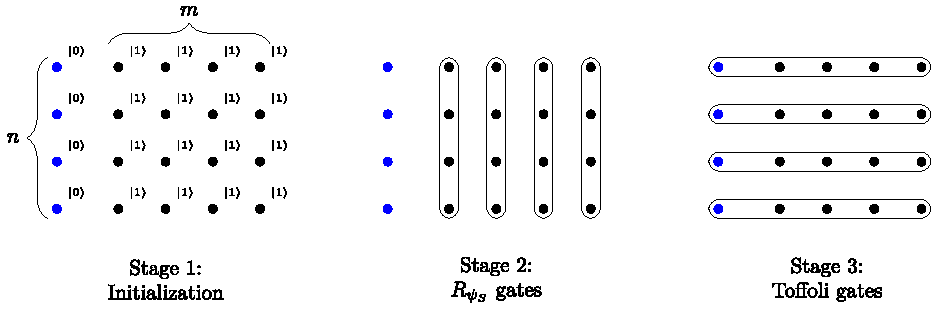
\includegraphics[width=\linewidth,height=0.78\textheight,keepaspectratio]{ccc2025-3-svg-01.pdf}\par

Figure 1: Constructing a nekomata from $U_{S}$ and Toffoli gates. Target qubits are shown in blue. Here $R_{\psi_{S}}$ is a rotation about the state $\left|\psi_{S}\right\rangle=\frac{1}{|S|}\sum_{x\in S}\left|x\right\rangle$ discussed further below.


% SOURCE-ID Thmtheorem19


\par\medskip\noindent\textbf{
\textbf{Theorem 19}\textbf{.}
}\par



\emph{For any parity-restricted $S\subseteq\{0,1\}^{n}$ with $|S|\leq 2^{n-4}$ there exists a depth-$4$, $O(n+\frac{2^{2n}}{|S|^{2}})$-size ${\mathsf{QAC}}_{S}$ circuit that constructs an $O(|S|^{2}2^{-2n})$-approximate nekomata.}\par



% END-SOURCE-ID Thmtheorem19




\par\medskip\noindent\textbf{Proof.}\par




The ${\mathsf{QAC}}_{S}$ circuit will act on $n(m+1)$ qubits arranged in a grid of width $m+1$ and height $n$. The first column will be designated as the “target” qubits, initialized to $\left|0^{n}\right\rangle$ and all other columns initialized to $\left|1^{n}\right\rangle$ (say, with a layer of $X$ gates). To each non-target column apply an $R_{\psi_{S}}=\mathbb{I}-2\left|\psi_{S}\right\rangle\!\left\langle\psi_{S}\right|$ gate, where $\left|\psi_{S}\right\rangle=H^{\otimes n}U_{S}H^{\otimes n}\left|0^{n}\right\rangle$. Note that this can be implemented in depth-$3$ as\par


\[\begin{gathered}
\mathbb{I}-2\left|\psi_{S}\right\rangle\!\left\langle\psi_{S}\right|=H^{\otimes n}U_{S}H^{\otimes n}(\mathbb{I}-2\left|0^{n}\right\rangle\!\left\langle 0^{n}\right|)H^{\otimes n}U_{S}H^{\otimes n}
\end{gathered}\]


which looks like the following quantum circuit:\par


\par\noindent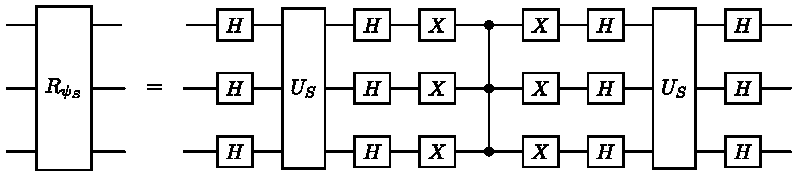
\includegraphics[width=\linewidth,height=0.78\textheight,keepaspectratio]{ccc2025-3-svg-02.pdf}\par


Finally, apply a Toffoli gate along each row with the output qubit being the corresponding target qubit (i.e. the qubit in the first column). We will now show that the probability that the target column is measured (in the computational basis) as $\left|b^{n}\right\rangle$ is at least $\frac{1}{2}-\frac{|S|}{2^{n-2}}$ for $b\in\{0,1\}$.\par




To start, let\par


\[\begin{gathered}
\displaystyle\gamma_{0}:=\left\langle 0^{n}\middle|\psi_{S}\right\rangle^{2} \displaystyle=\left\langle 0^{n}\right|H^{\otimes n}U_{S}H^{\otimes n}\left|0^{n}\right\rangle^{2} \\
\displaystyle=\bigg{[}\left\langle 0^{n}\right|\bigg{(}\left|0^{n}\right\rangle-\frac{1}{2^{n-1}}\sum_{s\in S}\sum_{x\in\{0,1\}^{n}}(-1)^{\langle x,s\rangle}\left|x\right\rangle\bigg{)}\bigg{]}^{2} \\
\displaystyle=\bigg{(}1-\frac{|S|}{2^{n-1}}\bigg{)}^{2}
\end{gathered}\]


and\par


\[\begin{gathered}
\displaystyle\gamma_{1}:=\left\langle 1^{n}\middle|\psi_{S}\right\rangle^{2} \displaystyle=\left\langle 1^{n}\right|H^{\otimes n}U_{S}H^{\otimes n}\left|0^{n}\right\rangle^{2} \\
\displaystyle=\bigg{[}\left\langle 1^{n}\right|\bigg{(}\left|0^{n}\right\rangle-\frac{2}{2^{n}}\sum_{s\in S}\sum_{x\in\{0,1\}^{n}}(-1)^{\langle x,s\rangle}\left|x\right\rangle\bigg{)}\bigg{]}^{2} \\
\displaystyle=\bigg{(}\frac{1}{2^{n-1}}\sum_{s\in S}(-1)^{|s|}\bigg{)}^{2} \\
\displaystyle=\frac{|S|^{2}}{2^{2n-2}}
\end{gathered}\]


where the last line follows from the fact that $S$ is parity-restricted. For $b\in\{0,1\}$, let $p_{b}$ be the probability that a given non-target column yields $\left|b^{n}\right\rangle$ after measuring in the computational basis. We have\par


\[\begin{gathered}
\displaystyle p_{0} \displaystyle=\left\langle 0^{n}\right|(\mathbb{I}-2\left|\psi_{S}\right\rangle\!\left\langle\psi_{S}\right|)\left|1^{n}\right\rangle^{2}=4\gamma_{0}\gamma_{1} \\
\displaystyle p_{1} \displaystyle=\left\langle 1^{n}\right|(\mathbb{I}-2\left|\psi_{S}\right\rangle\!\left\langle\psi_{S}\right|)\left|1^{n}\right\rangle^{2}=(1-2\gamma_{1})^{2}
\end{gathered}\]


Notice that, in fact, $\gamma_{1}$ is maximized when $S$ is parity-restricted (at least among sets of the same size as $S$). This, in turn, minimizes the probability that any given column is measured as $\left|1^{n}\right\rangle$ (though this will still be the most likely outcome since $|S|\leq 2^{n-4}$). Though, one may perform a similar analysis for sets $S$ which are only approximately parity-restricted.\par




Recall that after we’ve created these states along the column, we apply Toffoli gates along the rows. Let’s now compute the probability that we measure all zeroes or all ones on the first column. Note that computational basis measurements commute with Toffoli gates of any size, so in order for the targets to be measured as $\left|1^{n}\right\rangle$ all other columns must also be measured as $\left|1^{n}\right\rangle$. Let $m=\lfloor\frac{-\ln(2)}{2\ln(1-2\gamma_{1})}\rceil$, then\par


\[\begin{gathered}
\displaystyle\mathbb{P}[\text{Targets measure }\left|1^{n}\right\rangle] \displaystyle=(1-2\gamma_{1})^{2m} \\
\displaystyle>(1-2\gamma_{1})^{\frac{-\ln(2)}{\ln(1-2\gamma_{1})}+1} \\
\displaystyle=\frac{1}{2}(1-2\gamma_{1}) \\
\displaystyle=\frac{1}{2}-\frac{|S|^{2}}{2^{2n-2}}
\end{gathered}\]


Now, call a non-target column “bad” if it is measured as anything other than $\left|0^{n}\right\rangle$ or $\left|1^{n}\right\rangle$. Via a union bound,\par


\[\begin{gathered}
\displaystyle\mathbb{P}[\text{Some column is bad}]\leq m(1-p_{0}-p_{1}) \displaystyle=m(1-4\gamma_{0}\gamma_{1}-(1-2\gamma_{1})^{2}) \\
\displaystyle=4m\gamma_{1}(1-\gamma_{0}-\gamma_{1})
\end{gathered}\]


Observe that\par


\[\begin{gathered}
\frac{1}{2}(1-2\gamma_{1})=(1-2\gamma_{1})^{\frac{-\ln(2)}{\ln(1-2\gamma_{1})}+1}\leq(1-2\gamma_{1})^{2m}\leq\exp(-4m\gamma_{1}),
\end{gathered}\]


so $4m\gamma_{1}\leq-\ln(\frac{1}{2}-\gamma_{1})<1$ as $\gamma_{1}\leq\frac{1}{16}$. So,\par


\[\begin{gathered}
\displaystyle 4m\gamma_{1}(1-\gamma_{0}-\gamma_{1}) \displaystyle<1-\gamma_{0}-\gamma_{1} \\
\displaystyle\leq\frac{|S|}{2^{n-2}}
\end{gathered}\]


Thus, every column is good with probability at least $1-\frac{|S|}{2^{n-2}}$ and the targets are measured as $\left|0^{n}\right\rangle$ with probability at least $1-\frac{|S|}{2^{n-2}}-(\frac{1}{2}-\frac{|S|^{2}}{2^{2n-2}})\geq\frac{1}{2}-\frac{|S|}{2^{n-2}}$. By Lemma 18, the state produced is an $\frac{|S|}{2^{n-3}}$-approximate nekomata. Also, note that $m=\Theta(1/\gamma_{1})$, hence the circuit has size $O(n+m)=O(n+\frac{2^{2n}}{|S|^{2}})$.
$\blacktriangleleft$\par




Note that $|S|$ affects our construction in two \emph{distinct} ways. First, the bound we obtain on the probability that some non-target column is bad is proportional to the size of $S$, i.e., $\frac{|S|}{2^{n-2}}$. This exactly corresponds to the approximation guarantee on the final approximate nekomata state. In particular, this means that for very large parity-restricted sets the approximation guarantee becomes quite poor. On the other hand, we choose $m=\Theta(\frac{2^{2n-2}}{|S|^{2}})$ so that the entire grid is measured as $\left|1^{n}\right\rangle^{\otimes m}$ with probability very close to $\frac{1}{2}$. This means that the number of columns in the grid shrinks as $|S|$ grows. The main takeaway is that this construction results in a tradeoff between the quality of the approximate nekomata state and circuit size depending on $|S|$.\par




It may seem peculiar that we require $S$ to not be too large in Theorem 19, but this is indeed necessary. Intuition suggests that $U_{S}$ should approximate the parity gate better when $|S|$ approaches $2^{n-1}$. In some sense, this is true: if $|S|=2^{n-1}$, then $U_{S}$ exactly computes parity (or its negation) in the phase. In this extreme setting, unfortunately, $U_{S}$ ceases to be a useful multi-qubit gate, as it is simply $\pm Z^{\otimes n}$. Roughly, as $|S|$ grows too large, $U_{S}$ no longer becomes useful for preparing column-states with the peaked measurement distributions exploited in the grid construction as a result of how weakly entangling the $U_{S}$ gate becomes. However, if you weakly approximate parity as a classical reversible gate (instead of in the phase) there is another set of techniques which allow for very large parity-restricted gates to be bootstrapped to approximately compute parity. This is further discussed in Section 3.2.\par




It should also be noted that by applying $Z^{\otimes n}$ to $U_{S}$ yields $U_{T}$ where $T$ is a parity restricted set of size $2^{n-1}-|S|$, which can be used to achieve a similar grid construction with different size and accuracy parameters.\par




Finally, let’s compare our construction to that of Rosenthal [21], which only requires generalized Toffoli gates. If one takes $S$ to be a singleton set then $U_{S}$ is locally-equivalent to a generalized Toffoli gate and the resulting constructions have similar guarantees. However, one critical difference is the fact that the present construction has depth-$4$ while Rosenthal’s is only depth-$2$ since it uses column states $H^{\otimes n}U_{S}H^{\otimes n}\left|1^{n}\right\rangle$. Let us analyze roughly what goes wrong in the present construction if we were to use the same state. First, let $d_{S}:=\frac{|S|}{2^{n-1}}$ be the density of $S$. We have $d_{S}$ and $1-d_{S}$ are the amplitudes on the states $\left|0^{n}\right\rangle$ and $\left|1^{n}\right\rangle$, respectively. Following the previous analysis, we find that all columns measure $\left|1^{n}\right\rangle$ with probability $(1-d_{S})^{2m}$ and the probability that some column measures $\left|0^{n}\right\rangle$ is $1-(1-d_{S}^{2})^{m}$. This means that if $(1-d_{S})^{2m}\approx\frac{1}{2}$ then $m=\Theta(1/d_{S})$, but $(1-d_{S}^{2})^{m}$ tends to $1$ when $m=\Theta(1/d_{S})$, so it seems that a depth-$2$ construction just using Hadamard and $U_{S}$ gates may not be possible (at least with these techniques). However, it may be possible to obtain a depth-$2$ construction here by using some single-qubit gate other than the Hadamard (as Rosenthal does), but this will lead to a slightly more complicated analysis.\par



% SOURCE-ID Thmtheorem20


\par\medskip\noindent\textbf{
\textbf{Corollary 20}\textbf{.}
}\par



\emph{If $S\subset\{0,1\}^{*}$ is a parity-restricted set satisfying $\frac{2^{n}}{|S\cap\{0,1\}^{n}|}=O(n^{a})$ and $\frac{2^{n}}{|S\cap\{0,1\}^{n}|}=\Omega(n^{b})$ for some constants $a,b>0$ then ${\mathsf{BQAC}}^{0}_{S}\supseteq{\mathsf{BQNC}}^{0}_{wf}$.}\par



% END-SOURCE-ID Thmtheorem20




\par\medskip\noindent\textbf{Proof.}\par




Observe that the construction in Theorem 19 yields a constant-depth ${\mathsf{QAC}}_{S}$ circuit of size $O(n+\frac{2^{2n}}{|S\cap\{0,1\}^{n}|^{2}})=O(n+n^{2a})={\mathsf{poly}}(n)$ which prepares an $O(n^{-b})$-approximate nekomata on $n$ qubits. Via Lemma 16 this circuit can be leveraged to compute $\mathsf{F}_{n}$ with approximation error $O(n^{-b})$. Note that we can make the error an arbitrarily small polynomial by making the circuit polynomially larger. That is, suppose we want to construct an $O(n^{-c})$-approximate $n$-nekomata for some $c>b$. Simply use the construction above for an $n^{c/b}$-nekomata, but only use $n$ of the targets (i.e., any $n^{c/b}$-nekomata \emph{is} an $n$-nekomata for $c>b$). The circuit will have size $O(n^{ac/b})$ and error at most $O(n^{-c})$. Therefore, by Lemma 16, there are poly-size ${\mathsf{QAC}}_{S}^{0}$ circuits to compute Fanout to arbitrary polynomial precision, so ${\mathsf{BQAC}}^{0}_{S}\supseteq{\mathsf{BQNC}}^{0}_{wf}$.
$\blacktriangleleft$
Next, we argue that Threshold gates can be used to hit the “sweet spot” of Theorem 19. Namely, they correspond to parity-restricted sets of the right size to make the size and accuracy of the above construction polynomial.\par



% SOURCE-ID Thmtheorem21


\par\medskip\noindent\textbf{
\textbf{Corollary 21}\textbf{.}
}\par



${\mathsf{BQTC}}^{0}={\mathsf{BQNC}}^{0}_{wf}$\emph{}\par



% END-SOURCE-ID Thmtheorem21




\par\medskip\noindent\textbf{Proof.}\par




Without a loss of generality assume $n$ is even, otherwise this can be rectified with a single ancilla qubit. Let $S=\{x\in\{0,1\}^{n}\ :\ |x|=\frac{n}{2}\}$, i.e., $S$ is the Hamming slice of weight $\frac{n}{2}$. Note that $|x|=\frac{n}{2}$ if and only if $\operatorname{Maj}(x_{1},\dots,x_{n})=1$ and $\operatorname{Maj}(x_{1},\dots x_{n},0)=0$, thus the $U_{S}$ gate can be implemented in depth $2$ by applying $\operatorname{Maj}_{n}$ once to $\left|\psi\right\rangle$, tacking on an ancilla qubit set to $\left|0\right\rangle$ then applying another $\operatorname{Maj}_{n}$ gate to $\left|\psi\right\rangle\left|0\right\rangle$. In this case the circuit from Theorem 19 has size $s=O(n+\frac{2^{2n}}{|S|^{2}})$ and produces an $\epsilon=\frac{|S|}{2^{n-3}}$-approximate nekomata. Since\par


\[\begin{gathered}
\displaystyle\dbinom{n}{n/2}\in\bigg{[}\frac{2^{n}}{\sqrt{2n}},\frac{2^{n}}{\sqrt{n\pi/2}}\bigg{]}
\end{gathered}\]


via Stirling’s formula, it follows that $s=O(n)$ and $\epsilon=O(\frac{1}{\sqrt{n}})$. Via Corollary 20, ${\mathsf{BQTC}}^{0}={\mathsf{BQNC}}^{0}_{wf}$.
$\blacktriangleleft$\par



% SOURCE-ID Thmtheorem22


\par\medskip\noindent\textbf{
\textbf{Theorem 22}\textbf{.}
}\par



\emph{The following tasks are equivalent under ${\mathsf{QAC}}^{0}$ reductions:}\par


\begin{enumerate}


\item[] 
1. 


\emph{Preparation of }$\frac{1}{{\mathsf{poly}}(n)}$\emph{-approximate nekomata from the all zeros state and the inverse transformation for some polynomial }$p$\emph{}\par





\item[] 
2. 


\emph{Approximately computing }$\mathsf{Th}_{n,k}$\emph{ to error }$\frac{1}{{\mathsf{poly}}(n)}$\emph{ for any }$k={\mathsf{poly}}(n)$\emph{}\par





\item[] 
3. 


\emph{Approximately computing }$\mathsf{EX}_{2k-2,k-1}$\emph{ to error }$\frac{1}{{\mathsf{poly}}(n)}$\emph{ for any }$k={\mathsf{poly}}(n)$\emph{}\par





\end{enumerate}



% END-SOURCE-ID Thmtheorem22




\par\medskip\noindent\textbf{Proof.}\par




Observe that for $x\in\{0,1\}^{2k-2}$ $\mathsf{Ex}_{2k-2,k-1}(x)=\mathsf{Th}_{2k-2,k-1}(x)\land\overline{\mathsf{Th}_{2k-2,k}(x)}$ and we can implement this directly by first applying $U$ to $\left|x\right\rangle\left|10^{n-(2k-2)-1}\right\rangle$ and then to $\left|x\right\rangle\left|0^{n-(2k-2)}\right\rangle$ for any $U$ which computes $\mathsf{Th}_{n,k}$ to inverse-polynomial precision. Thus, (2) $\implies$ (3).\par




Via Theorem 19 a unitary $V$ approximately computes $\mathsf{EX}_{2k-2,k-1}$ to inverse-polynomial error can be leveraged in constant-depth to prepare an $\frac{1}{{\mathsf{poly}}(k)}$-approximate nekomata on $k$ qubits. In fact, this construction will yield an approximate nekomata on $2k-2$ qubits, but as mentioned in the proof of Corollary 20, an approximate nekomata on $2k-2$ is also an approximate nekomata on $k$ qubits. This circuit (and the inverse transformation) can be used to compute $\mathsf{F}_{k}$ to the same precision, up to constants (Lemma 16). Observe that iteratively applying $\mathsf{F}_{k}$ in a tree-like fashion allows us to apply fanout to a number of qubits that is exponential in the depth. In particular, using $\mathsf{F}_{k}$ gates we can construct $\mathsf{F}_{k^{d}}$ in depth $d$ by stacking $\mathsf{F}_{k}$ gates on the qubits which we have fanned-out onto in the previous layer (see Figure 2). This means that as long as $k=n^{\alpha}$ for some $\alpha=\Omega(1)$ we can take $d=O(1/\alpha)=O(1)$ and approximately compute $\mathsf{F}_{n}$ to the same precision. Hence, (3) $\implies$ (1).\par




Finally, (1) $\implies$ (2) can be seen by applying the construction of [13] which allows us to approximately compute any threshold gate on ${\mathsf{poly}}(n)$ qubits via a ${\mathsf{QNC}}^{0}_{wf}$ circuit.
$\blacktriangleleft$\par



\par\noindent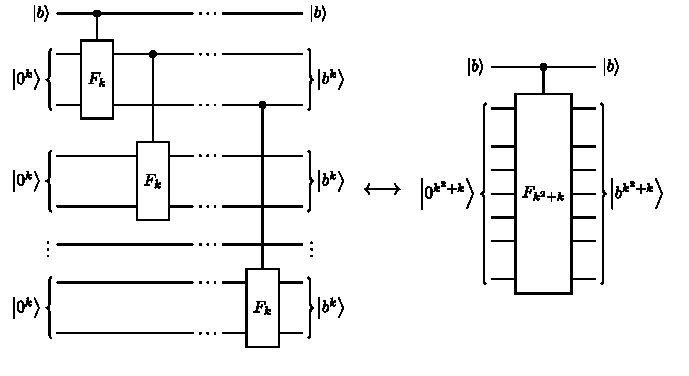
\includegraphics[width=\linewidth,height=0.78\textheight,keepaspectratio]{ccc2025-3-svg-03.pdf}\par

Figure 2: Iteratively applying $F_{k}$ in a tree-like fashion. In the above, we achieve fanout $k^{2}+k$ in depth-$2$ using $F_{k}$ gates.





\par\medskip\noindent\textbf{
3.2 Removing the Toffoli gates}\par




The construction presented in Theorem 19 for generic $S$ requires large Toffoli gates, however we will show that for some regimes of $|S|$, these gates are unnecessary, i.e., ${\mathsf{QNC}}^{0}_{S}$ circuits can exactly compute Toffoli on polynomially many qubits. We will show that this is indeed the case when $|S|\geq 2^{n-O(1)}$ and $|S|\leq 2^{(1-\epsilon)n}$ for a fixed constant $\epsilon<1$. Though for this result we require the use of $U_{f_{S}}$ gates, i.e., those gates which check membership in $S$ as $U_{f_{S}}\left|x\right\rangle\left|b\right\rangle=\left|x\right\rangle\left|f(x)\oplus b\right\rangle$ where $f(x)=1$ iff $x\in S$.\par



% SOURCE-ID Thmtheorem23


\par\medskip\noindent\textbf{
\textbf{Lemma 23}\textbf{.}
}\par



\emph{Let $c$ be constant, and let $S$ be a parity restricted set with size $|S|\geq 2^{n-c}$ and strings of parity $b\in\{0,1\}$. Then, there exist some $c-1$ bit-strings $t_{1},t_{2},\dots t_{c-1}\in\{0,1\}^{n}$ such that $|x|\equiv b\pmod{2}$ iff}\par


\[\begin{gathered}
\displaystyle\bigvee_{y\in\mathrm{Span}(t_{1},\dots t_{c-1})}\{x\oplus y\in S\}
\end{gathered}\]


\emph{is satisfied.}\par



% END-SOURCE-ID Thmtheorem23



\par\medskip\noindent\textbf{Proof.}\par




Suppose that $b=0$. Let $\mathcal{E}\subset\mathbb{F}_{2}^{n}$ be the subspace of dimension $n-1$ consisting of vectors of even Hamming weight. Observe that $S\subseteq\mathcal{E}$, and moreover that $S$ contains at least $n-c$ linearly independent elements of $\mathcal{E}$. Therefore, there exist some $t_{1},\cdots t_{c-1}\in\mathcal{E}$ such that $S\cup\{t_{1},\dots t_{c-1}\}$ span $\mathcal{E}$. Hence, every element of $\mathcal{E}$ can be written as $s\oplus y$ for some $s\in S$ and $y\in\text{span}\{t_{1},\dots t_{c-1}\}$. Thus, $|x|\equiv 0$ iff the disjunction is satisfied.\par




If $b=1$ then the set $S^{\prime}$ obtained by flipping the first bit of every element of $S$ contains vectors of even Hamming weight - further, $S^{\prime}$ contains at least $n-c$ linearly independent vectors. So, take $\{t_{1},\dots t_{c-1}\}$ as before such that $S^{\prime}\cup\{t_{1},\dots t_{c-1}\}$ spans $\mathcal{E}$. Any vector of even Hamming weight, $y\in\mathbb{F}_{2}^{n}$, can be expressed as $y=s^{\prime}+t^{\prime}$ for some $s^{\prime}\in S^{\prime}$ and $t^{\prime}\in\text{Span}(t_{1},\dots t_{c-1})$. Now, observe that if $x=(x_{1},\dots x_{n})\in\mathbb{F}_{2}^{n}$ has odd Hamming weight then $(x_{1}\oplus 1,\dots x_{n})$ can be expressed as $s^{\prime}+t^{\prime}$ for some $s^{\prime}\in S^{\prime}$ and $t^{\prime}\in\text{Span}(t_{1},\dots t_{c-1})$. Since $s^{\prime}=(s_{1}\oplus 1,s_{2},\dots s_{n})$ for some $s=(s_{1},s_{2},\dots s_{n})\in S$, it follows that $x$ has odd Hamming weight iff the disjunction is satisfied.
$\blacktriangleleft$
As shown above, if $|S|\geq 2^{n-c}$ for some constant $c$ then we can extend $S$ linearly to “cover” all strings of a fixed Hamming weight. To implement a parity gate in this way, one can encode every linear combination $t^{\prime}\in\text{Span}(t_{1},\dots t_{c})$ in the ancilla and then apply a $U_{f_{S}}$ gate to $\left|x\oplus t^{\prime}\right\rangle$ for every $t^{\prime}$ - this can be done in constant depth using only $U_{f_{S}}$ and $\mathsf{CNOT}$ gates since $|\text{Span}(t_{1},\dots t_{c})|=2^{c}=O(1)$. If any of these $U_{f_{S}}$ gates evaluate to $1$ then $x$ must have Hamming weight consistent with that of the strings in $S$, in effect computing the parity of $x$. We will now see how generalized Toffoli can be computed with just $U_{f_{S}}$ and $\mathsf{CNOT}$ gates when $|S|$ is sufficiently small.\par



% SOURCE-ID Thmtheorem24


\par\medskip\noindent\textbf{
\textbf{Lemma 24}\textbf{.}
}\par



\emph{For any $S\subseteq\{0,1\}^{n}$ there exists some $s\in S$ and some subset of indices $\{i_{1},i_{2},\dots i_{k}\}$ such that $s$ is the unique $x\in S$ which satisfies
$x_{i_{j}}=s_{i_{j}}$ for all $j\in[k]$. Further, $k\leq\log{|S|}$.}\par



% END-SOURCE-ID Thmtheorem24




\par\medskip\noindent\textbf{Proof.}\par




Note that unless $|S|=1$ there exists some index on which elements of $S$ take different values. If $|S|=1$ we are done and can take this single element to be $s$. Otherwise, let $i_{1}$ be the first index on which elements of $S$ take different values. We will now partition $S$ into two sets $S^{1}_{0}$ and $S^{1}_{1}$ where $S^{1}_{b}=\{s\in S\ |\ s_{i_{1}}=b\}$. Take $T_{1}$ to be the set with fewer elements and repeat this procedure, defining $T_{j}$ similarly for $j>1$. Since $|T_{j+1}|\leq\frac{|T_{j}|}{2}$ for $j\geq 1$, it follows that for some $k>1$, $|T_{k}|=1$ and it follows that $k\leq\log{|S|}$.
$\blacktriangleleft$
Now, when $|S|$ is sufficiently small, there is always some way to fix a small number ($\log|S|$) of bits so that the unfixed bits have a unique assignment consistent with $S$. In particular, if $|S|\leq 2^{(1-\epsilon)n}$ for some constant $\epsilon\in(0,1)$ then there exists some partial assignment of at most $(1-\epsilon)n$ bits such that for the remaining $\epsilon n$ bits there is a unique assignment such that the resulting string is a member of $S$. For simplicity, suppose that the partial assignment is on the first $(1-\epsilon)n$ as $y\in\{0,1\}^{(1-\epsilon)n}$ and that the unique assignment for the remaining bits which is consistent with $S$ is $z\in\{0,1\}^{\epsilon n}$. Now, for $x\in\{0,1\}^{\epsilon n}$ we can see that\par


\[\begin{gathered}
\displaystyle U_{f_{S}}\left|y\right\rangle\left|x\right\rangle\left|0\right\rangle=\left|y\right\rangle\left|x\right\rangle\left|\mathbb{I}_{z}(x)\right\rangle
\end{gathered}\]


In this way, after fixing the first $(1-\epsilon)n$ bits to $y$ forces $U_{f_{S}}$ to act like a $U_{f_{\{z\}}}$ gate on the remaining qubits. This gate is locally equivalent to a Toffoli gate; we can just apply $X$ gates to the wires on which $z_{i}=0$. Since $\epsilon$ is a constant, we can repeat this procedure $1/\epsilon$ times to implement the Toffoli gate on $n$ qubits in constant depth. In this way, we can directly implement generalized Toffoli gates in the grid construction of Theorem 19 using the $U_{f_{S_{n}}}$ gates when $|S|$ is sufficiently small.\par



% SOURCE-ID Thmtheorem25


\par\medskip\noindent\textbf{
\textbf{Corollary 25}\textbf{.}
}\par



\emph{For any parity restricted set $S$ which satisfies $|S|\geq\Omega(2^{n})$ or $|S|\leq 2^{(1-\epsilon)n}$ for some fixed $\epsilon\in(0,1)$ there exist constant-depth ${\mathsf{QNC}}_{S}$ circuits of size $O(n+\frac{2^{2n}}{|S|^{2}})$ which prepare $O(\frac{|S|^{2}}{2^{2n}})$-approximate nekomata. In particular, for $S\subset\{0,1\}^{*}$ which are parity restricted and satisfy $\frac{2^{n}}{|S\cap\{0,1\}^{n}|}={\mathsf{poly}}(n)$, ${\mathsf{BQNC}}^{0}_{S}\supseteq{\mathsf{BQNC}}^{0}_{wf}$.}\par



% END-SOURCE-ID Thmtheorem25






\par\medskip\noindent\textbf{
4 Quantum MOD gates are powerful even on their own}\par




In this section we show a strengthening of a result of [8]. In particular they show that for any fixed $q>1$ $\mathsf{MOD}_{n,q}$ gates, $\wedge_{n}$ gates, single- and two-qubit gates can be leveraged to implement Fanout in constant depth and polynomial size:\par



% SOURCE-ID Thmtheorem26


\par\medskip\noindent\textbf{
\textbf{Theorem 26}\textbf{ }(Theorem 4.6 of [8])\textbf{.}
}\par



\emph{For $p\geq 2$, ${\mathsf{QAC}}^{0}[p]={\mathsf{QAC}}^{0}_{wf}$.}\par



% END-SOURCE-ID Thmtheorem26



However, the family of ${\mathsf{QAC}}^{0}[p]$ circuits they construct does not actually require $\wedge_{n}$ gates, i.e., the family of circuits they construct to compute $\mathsf{F}_{n}$ is actually a ${\mathsf{QNC}}^{0}[p]$ family. This immediately yields the collapse of all ${\mathsf{QNC}}^{0}[p]$:\par




% SOURCE-ID Thmtheorem27


\par\medskip\noindent\textbf{
\textbf{Theorem 27}\textbf{.}
}\par



${\mathsf{QNC}}^{0}[p]={\mathsf{QNC}}^{0}_{wf}$\emph{ for all primes $p$.}\par



% END-SOURCE-ID Thmtheorem27




Combined with the results of [13] and [24] we have an even larger collapse of constant-depth circuit classes:\par


\[\begin{gathered}
{\mathsf{QNC}}^{0}[p]={\mathsf{QNC}}^{0}_{wf}={\mathsf{QAC}}^{0}_{wf}={\mathsf{QAC}}^{0}[q]={\mathsf{QTC}}^{0}_{wf}
\end{gathered}\]


for all $p,q\geq 2$. Before showing and analyzing the construction we will introduce some preliminaries.\par




\par\medskip\noindent\textbf{
4.1 Simulating qudit arithmetic in ${\mathsf{QNC}}^{0}[p]$
}\par




By a proposition of Moore, in order to inplement $\mathsf{F}_{n}$ it actually suffices to construct a circuit which behaves like $\mathsf{F}_{n}$ when all but the one qubit to be fanned-out are set to $\left|0\right\rangle$:\par



% SOURCE-ID Thmtheorem28


\par\medskip\noindent\textbf{
\textbf{Proposition 28}\textbf{ }(Proposition 1 of [17])\textbf{.}
}\par



\emph{In any class of quantum circuits which includes Hadamard and $\mathsf{CNOT}$-gates, the follow are equivalent in constant depth:}\par


\begin{enumerate}


\item[] 
1. 


\emph{It is possible to map }$(\alpha\left|0\right\rangle+\beta\left|1\right\rangle)\left|0^{n-1}\right\rangle$\emph{ to }$\alpha\left|0^{n}\right\rangle+\beta\left|1^{n}\right\rangle$\emph{ and from }$\alpha\left|0^{n}\right\rangle+\beta\left|1^{n}\right\rangle$\emph{ to }$(\alpha\left|0\right\rangle+\beta\left|1\right\rangle)\left|0^{n-1}\right\rangle$\emph{ for all }$|\alpha|^{2}+|\beta|^{2}=1$\emph{}\par





\item[] 
2. 


$\mathsf{F}_{n}$\emph{ can be implemented with at most }$n-1$\emph{ ancilla qubits}\par





\item[] 
3. 


${\mathsf{P}}_{n}$\emph{ can be implemented with at most }$n-1$\emph{ ancilla qubits}\par





\end{enumerate}



% END-SOURCE-ID Thmtheorem28



Hence, constructing a unitary $U$ which satisfies $U(\alpha\left|0\right\rangle+\beta\left|1\right\rangle)\otimes\left|0^{n-1+a(n)}\right\rangle=(\alpha\left|0^{n}\right\rangle+\beta\left|1^{n}\right\rangle)\left|0^{a(n)}\right\rangle$ for any single-qubit state $\alpha\left|0\right\rangle+\beta\left|1\right\rangle$ will result in the ability to compute Fanout; this is exactly what the construction does.\par




First, for a fixed prime $p$ consider the qudit generalizations of the Parity and Fanout gates for local dimension $p$:\par


\[\begin{gathered}
\displaystyle\mathsf{M}_{n,p}\left|b\right\rangle\left|x_{1}x_{2}\cdots x_{n}\right\rangle \displaystyle=\left|b-|x|\mod{p}\right\rangle\left|x_{1}x_{2}\cdots x_{n}\right\rangle \\
\displaystyle\mathsf{F}_{n,p}\left|b\right\rangle\left|x_{1}x_{2}\cdots x_{n}\right\rangle \displaystyle=\left|b\right\rangle\left|(x_{1}+b\mod{p}),(x_{2}+b\mod{p}),\ldots,(x_{n}+b\mod{p})\right\rangle
\end{gathered}\]


where $x_{1},\ldots,x_{n},b\in\{0,\dots p-1\}$.\par




Additionally, consider the following single-qudit gate:\par


\[\begin{gathered}
\displaystyle Q_{p}\left|b\right\rangle=\frac{1}{\sqrt{p}}\sum_{j=0}\omega^{jb}\left|j\right\rangle
\end{gathered}\]


where $\omega=e^{2i\pi/p}$. For example, when $p=2$, $Q_{p}=H$, and $\mathsf{F}_{n,p}$ and $\mathsf{M}_{n,p}$ are the usual Fanout and Parity gates for qubits, respectively.\par



% SOURCE-ID Thmtheorem29


\par\medskip\noindent\textbf{
\textbf{Lemma 29}\textbf{ }(Proposition 4.2 of [8])\textbf{.}
}\par



$\mathsf{M}_{n,p}=(Q_{p}^{{\dagger}})^{\otimes(n+1)}\mathsf{F}_{n,p}Q_{p}^{\otimes(n+1)}$\emph{}\par



% END-SOURCE-ID Thmtheorem29



Recall our goal: we want to use Mod-$p$ gate to simulate Fanout over qubits. While this seems somewhat challenging for qubits, it is trivial over qudits of local dimension $p$ by Lemma 29. Therefore, our plan will be to pretend that we are in that setting by encoding a qudit using several qubits. Once we have set an encoding, we need encoded versions of the $\mathsf{M}_{n,p}$ and $Q_{p}$ gates in Lemma 29. Encoding the $Q_{p}$ gate is easy – it’s a gate of constant-size and each one of our encoded qudits will be of constant size, so any brute force encoding of $Q_{p}$ will do. The challenging step is to show that an encoded $\mathsf{M}_{n,p}$ gate is possible using (qubit) $\mathsf{MOD}_{n,p}$ gates. One of the key observations is that after we’ve applied the encoded Fanout, we will have accomplished Task 1 of Proposition 28, and therefore, we can construct general Fanout over qubits.\par




\par\medskip\noindent\textbf{Proof of Theorem 27.}\par




To start, define a linear encoding map $E\colon\mathbb{C}^{p}\to(\mathbb{C}^{2})^{\otimes p}$ which maps from qudits of local dimension $p$ to a tensor product of $p$ qubits:\par


\[\begin{gathered}
\displaystyle E\left|j\right\rangle=\bigotimes_{k=0}^{p-1}\left|\delta_{k,j}\right\rangle
\end{gathered}\]


for all $j\in\{0,\ldots,p-1\}$ and where $\delta_{k,j}$ denotes the Kronecker delta function. Note that $E$ is a linear map of full rank from the $p$-dimensional space spanned by $\{\left|j\right\rangle\}_{j=0}^{p-1}$ to the $p$-dimensional subspace of $(\mathbb{C}^{2})^{\otimes n}$ spanned by$\bigg{\{}\bigotimes_{k=0}^{p-1}\left|\delta_{k,j}\right\rangle\bigg{\}}_{j=0}^{p-1}$. Throughout this construction we will only be working over qubits and not actually implementing $E$. Instead, we will be exploiting the equivalence of Lemma 29 by simulating qudit arithmetic with qubits. We introduce $E$ for the sake of describing this simulation method succinctly.\par




Now, applying $Q_{p}$ to an encoded state on qubits amounts to implementing any $\tilde{Q}_{p}$ which satisfies:\par


\[\begin{gathered}
\tilde{Q}_{p}\left|\delta_{0,j}\right\rangle\left|\delta_{1,j}\right\rangle\cdots\left|\delta_{p-1,j}\right\rangle=\frac{1}{\sqrt{p}}\sum_{k=0}^{p-1}\omega^{jk}\left|\delta_{0,k}\right\rangle\left|\delta_{1,k}\right\rangle\cdots\left|\delta_{p-1,k}\right\rangle
\end{gathered}\]


i.e., any unitary $\tilde{Q}_{p}$ on $(\mathbb{C}^{2})^{\otimes p}$ which respects the homomorphism induced by $E$. Since $p$ is fixed, any such $\tilde{Q}_{p}$ operates on constantly many qubits and can be implemented in constant depth and size.\par




Now, we must implement $\mathsf{M}_{n,p}$ on the encoded subspace using just $\mathsf{MOD}_{n,p}$ (and one- and two-qubit gates). Note that for any $j_{1},\dots j_{n}\in\mathbb{F}_{p}$ their sum modulo $p$ can be decomposed






$\displaystyle j_{1}+\cdots+j_{n}$
$\displaystyle\equiv 0(\delta_{0,j_{1}}+\cdots+\delta_{0,j_{n}})+1(\delta_{1,j_{1}}+\cdots+\delta_{1,j_{n}})+\cdots+(p-1)(\delta_{p-1,j_{1}}+\cdots+\delta_{p-1,j_{n}})$




$\displaystyle\equiv\sum_{k=0}^{p-1}k\bigg{(}\sum_{i=1}^{n}\delta_{k,j_{i}}\bigg{)}\pmod{p}$




Let $s_{k}:=\sum_{i=1}^{n}\delta_{k,j_{i}}\pmod{p}$ be the number of $j_{i}$ terms equal to $k$ modulo $p$. Let’s also define a family of generalized Mod-$p$ gates over qubits.
For $\ell\in\{0,\dots p-1\}$, recall $\mathsf{MOD}_{n,p,\ell}$ acts as\par


\[\begin{gathered}
\displaystyle\mathsf{MOD}_{n,p,\ell}\left|b\right\rangle\left|x_{1},\dots x_{n}\right\rangle=\left|b\oplus{\mathsf{Mod}}_{n,p,\ell}(x)\right\rangle\left|x_{1},\dots x_{n}\right\rangle
\end{gathered}\]




Notice that $\mathsf{MOD}_{n,p,\ell}$ can be implemented over qubits with an $\mathsf{MOD}_{n,p,0}$ gate (the standard $\mathsf{MOD}_{n,p}$ gate on qubits) and $p-1$ additional ancilla qubits, $p-\ell$ of which are set to $1$. We can use these gates to compute $s_{k}$ for a given $k\in\{0,1\dots p-1\}$:\par


\par\noindent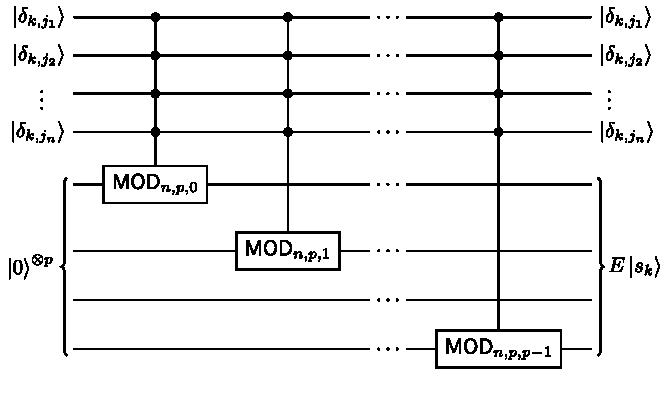
\includegraphics[width=\linewidth,height=0.78\textheight,keepaspectratio]{ccc2025-3-svg-04.pdf}\par


For $k\in\{0,\dots p-1\}$ the above circuit, can be applied in parallel to the appropriate qubits in the encoding; namely those of the form $\left|\delta_{k,j}\right\rangle$ for fixed $k$. This leaves us with the state $E\left|s_{0}\right\rangle\otimes\cdots\otimes E\left|s_{p-1}\right\rangle$. Recall that the sum over $\mathbb{F}_{p}$ we wish to compute is $\sum_{i=1}^{n}j_{i}=\sum_{k=0}^{p-1}ks_{k}$; so, if we can compute each of $ks_{k}$ and sum over all $k$, we will be left with the desired sum. However, the product $ks_{k}$ is over elements of $\mathbb{F}_{p}$ and $p$ is fixed, so it is clear that this can be computed in ${\mathsf{QNC}}^{0}$ (${\mathsf{NC}}^{0}$ even). Further, $\sum_{k=0}^{p-1}ks_{k}$ is a sum of constantly many integers each described by $p=O(1)$ bits, which is of course computable by a ${\mathsf{QNC}}^{0}$ (${\mathsf{NC}}^{0}$ even) circuit.\par




For the sake of completeness, we will describe a circuit composed of permutations on $p$ qubits which computes $\sum_{k=0}^{p-1}ks_{k}$ in our encoded subspace. First let $U_{\sigma}$ be the permutation unitary which satisfies $U_{\sigma}E\left|j\right\rangle=E\left|j-1\mod{p}\right\rangle$. For any $k\in\{0,1,\dots p-1\}$, $U_{\sigma}^{k}$ can be implemented in constant depth via a sequence of at most $p^{2}$ swap gates. Since $U_{\sigma}^{a}E\left|j\right\rangle=E\left|j-a\right\rangle$ for all $a,j\in\mathbb{F}_{p}$, we can in series apply $U_{\sigma}^{ks_{k}}$ to $E\left|b\right\rangle$ to finally achieve\par




\[\begin{gathered}
\displaystyle\bigg{(}\prod_{k=0}^{p-1}U_{\sigma}^{ks_{k}}\bigg{)}E\left|b\right\rangle \displaystyle=U_{\sigma}^{\sum_{k=0}^{p-1}ks_{k}}E\left|b\right\rangle \\
\displaystyle=U_{\sigma}^{\sum_{i=1}^{n}j_{i}}\left|b\right\rangle \\
\displaystyle=E\left|b-\sum_{i=1}^{n}j_{i}\mod{p}\right\rangle
\end{gathered}\]


Hence, this gives a circuit of depth $p^{3}=O(1)$ and linear size for simulating $\mathsf{M}_{p,n}$ on the encoded qudits. After conjugating by $\tilde{Q}_{p}$ gates on the appropriate groups of qubits the equivalence of Lemma 29 shows that the entire circuit exactly implements fanout on the encoded qudits.\par




Let’s now put all the pieces together to show that we can achieve Task 1 of Proposition 28. Starting with the state $(\alpha\left|0\right\rangle+\beta\left|1\right\rangle)\left|0^{(p(n+1)-1)}\right\rangle$, we want to get to an \emph{encoding} of $\alpha\left|0\right\rangle+\beta\left|1\right\rangle$ and the ancillary qubits. First, apply a $\mathsf{CNOT}$ gate from the first to second qubit, followed by an $X$ gate on the first to obtain the state\par


\[\begin{gathered}
\displaystyle(\alpha\left|10^{p-1}\right\rangle+\beta\left|010^{p-2}\right\rangle)\otimes\left|0^{pn}\right\rangle.
\end{gathered}\]


Now apply an $X$ gate to the $(pj+1)$st qubit for $j\in\{0,1,\dots n-1\}$ yielding the encoded state: $E(\alpha\left|0\right\rangle+\beta\left|1\right\rangle)\otimes E\left|0^{n}\right\rangle$. Note that this is a state on $n+1$ \emph{qudits} encoded by $p(n+1)$ \emph{qubits}. After applying the previously described circuit which simulates $\mathsf{F}_{n,p}$ on the encoded states the result is (up to a known permutation of the qubits)\par


\[\begin{gathered}
\displaystyle(\alpha\left|0\right\rangle^{\otimes 2(n+1)}+\beta\left|1\right\rangle^{\otimes 2(n+1)})\otimes\left|0^{(p-2)(n+1)}\right\rangle
\end{gathered}\]


Now, via Proposition 28 any such circuit is sufficient to compute Fanout (on qubits), thus ${\mathsf{QNC}}^{0}_{wf}\subseteq{\mathsf{QNC}}^{0}[p]$. It is shown in [13] and [24] that the reverse inclusion holds and it can be concluded that ${\mathsf{QNC}}^{0}_{wf}={\mathsf{QNC}}^{0}[p]$.
$\blacktriangleleft$\par



% SOURCE-ID Thmtheorem30


\par\medskip\noindent\textbf{
\textbf{Corollary 30}\textbf{.}
}\par



${\mathsf{QNC}}^{0}[a]={\mathsf{QNC}}^{0}_{wf}$\emph{ for all $a>1$.}\par



% END-SOURCE-ID Thmtheorem30




\par\medskip\noindent\textbf{Proof.}\par




This follows from the previous construction by taking $p$ to be any prime factor of $a$ and setting ancilla qubits appropriately or concatenating the input $a/p$ times so that any $\mathsf{MOD}_{a}$ gate instead computes $\mathsf{MOD}_{p}$.
$\blacktriangleleft$\par







\par\medskip\noindent\textbf{References}\par



\begin{itemize}


\item[] 
[1]

Miklós Ajtai.


$\Sigma_{1}$-formulae on finite structures.


\emph{Annals of pure and applied logic}, 24(1):1–48, 1983.





\item[] 
[2]

Anurag Anshu, Yangjing Dong, Fengning Ou, and Penghui Yao.


On the computational power of ${\mathsf{QAC}}^{0}$ with barely superlinear
ancillae.


\emph{arXiv preprint}, 2024.


arXiv:2410.06499.





\item[] 
[3]

Debajyoti Bera.


A lower bound method for quantum circuits.


\emph{Information processing letters}, 111(15):723–726, 2011.


doi:10.1016/J.IPL.2011.05.002.





\item[] 
[4]

Sergey Bravyi, David Gosset, and Robert König.


Quantum advantage with shallow circuits.


\emph{Science}, 362(6412):308–311, 2018.





\item[] 
[5]

Harry Buhrman, Marten Folkertsma, Bruno Loff, and Niels MP Neumann.


State preparation by shallow circuits using feed forward.


\emph{arXiv preprint}, 2023.


arXiv:2307.14840.





\item[] 
[6]

Maosen Fang, Stephen Fenner, Frederic Green, Steven Homer, and Yong Zhang.


Quantum lower bounds for fanout.


\emph{Quantum Information and Computation}, 6(1):046–057, 2006.


doi:10.26421/QIC6.1-3.





\item[] 
[7]

Merrick Furst, James B Saxe, and Michael Sipser.


Parity, circuits, and the polynomial-time hierarchy.


\emph{Mathematical systems theory}, 17(1):13–27, 1984.


doi:10.1007/BF01744431.





\item[] 
[8]

Frederic Green, Steven Homer, Cristopher Moore, and Christopher Pollett.


Counting, fanout, and the complexity of quantum ${\mathsf{ACC}}$.


\emph{arXiv preprint}, 2001.


arXiv:quant-ph/0106017.





\item[] 
[9]

Daniel Grier and Luke Schaeffer.


Interactive shallow clifford circuits: quantum advantage against
nc1 and beyond.


In \emph{Proceedings of the 52nd Annual ACM SIGACT Symposium on Theory
of Computing}, pages 875–888, 2020.


doi:10.1145/3357713.3384332.





\item[] 
[10]

Alex Bredariol Grilo, Elham Kashefi, Damian Markham, and Michael de Oliveira.


The power of shallow-depth Toffoli and qudit quantum circuits.


\emph{arXiv preprint}, 2024.


doi:10.48550/arXiv.2404.18104.





\item[] 
[11]

Jonas Haferkamp, Dominik Hangleiter, Adam Bouland, Bill Fefferman, Jens Eisert,
and Juani Bermejo-Vega.


Closing gaps of a quantum advantage with short-time hamiltonian
dynamics.


\emph{Physical Review Letters}, 125(25):250501, 2020.





\item[] 
[12]

Johan Håstad.


\emph{Computational limitations for small depth circuits}.


PhD thesis, Massachusetts Institute of Technology, 1986.





\item[] 
[13]

Peter Høyer and Robert Špalek.


Quantum fan-out is powerful.


\emph{Theory of computing}, 1(1):81–103, 2005.


doi:10.4086/TOC.2005.V001A005.





\item[] 
[14]

Harry Levine, Alexander Keesling, Giulia Semeghini, Ahmed Omran, Tout T Wang,
Sepehr Ebadi, Hannes Bernien, Markus Greiner, Vladan Vuletić, Hannes
Pichler, et al.


Parallel implementation of high-fidelity multiqubit gates with
neutral atoms.


\emph{Physical review letters}, 123(17):170503, 2019.





\item[] 
[15]

Nathan Linial, Yishay Mansour, and Noam Nisan.


Constant depth circuits, fourier transform, and learnability.


\emph{Journal of the ACM (JACM)}, 40(3):607–620, 1993.


doi:10.1145/174130.174138.





\item[] 
[16]

Klaus Mølmer and Anders Sørensen.


Multiparticle entanglement of hot trapped ions.


\emph{Physical Review Letters}, 82(9):1835, 1999.





\item[] 
[17]

Cristopher Moore.


Quantum circuits: Fanout, parity, and counting.


\emph{arXiv preprint}, 1999.


arXiv:quant-ph/9903046.





\item[] 
[18]

Shivam Nadimpalli, Natalie Parham, Francisca Vasconcelos, and Henry Yuen.


On the pauli spectrum of ${\mathsf{QAC}}^{0}$.


In \emph{Proceedings of the 56th Annual ACM Symposium on Theory of
Computing}, pages 1498–1506, 2024.





\item[] 
[19]

Daniel Padé, Stephen Fenner, Daniel Grier, and Thomas Thierauf.


Depth-2 ${\mathsf{QAC}}$ circuits cannot simulate quantum parity.


\emph{arXiv preprint}, 2020.


arXiv:2005.12169.





\item[] 
[20]

Alexander A Razborov.


Lower bounds on the size of bounded depth circuits over a complete
basis with logical addition.


\emph{Mat. Zametki}, 41(4):598–607, 1987.





\item[] 
[21]

Gregory Rosenthal.


Bounds on the ${\mathsf{QAC}}^{0}$ complexity of approximating parity.


In \emph{12th Innovations in Theoretical Computer Science Conference
(ITCS 2021)}. Schloss Dagstuhl – Leibniz Zentrum für Informatik, 2021.


doi:10.4230/LIPIcs.ITCS.2021.32.





\item[] 
[22]

Mark Saffman and Klaus Mølmer.


Efficient multiparticle entanglement via asymmetric Rydberg
blockade.


\emph{Physical review letters}, 102(24):240502, 2009.





\item[] 
[23]

Roman Smolensky.


Algebraic methods in the theory of lower bounds for Boolean circuit
complexity.


In \emph{Proceedings of the nineteenth annual ACM symposium on Theory
of computing}, pages 77–82, 1987.


doi:10.1145/28395.28404.





\item[] 
[24]

Yasuhiro Takahashi and Seiichiro Tani.


Collapse of the hierarchy of constant-depth exact quantum circuits.


\emph{computational complexity}, 25:849–881, 2016.


doi:10.1007/S00037-016-0140-0.





\item[] 
[25]

Barbara M Terhal and David P DiVincenzo.


Adaptive quantum computation, constant depth quantum circuits and
arthur-merlin games.


\emph{arXiv preprint}, 2002.


arXiv:quant-ph/0205133.





\item[] 
[26]

Adam Bene Watts, Robin Kothari, Luke Schaeffer, and Avishay Tal.


Exponential separation between shallow quantum circuits and unbounded
fan-in shallow classical circuits.


In \emph{Proceedings of the 51st Annual ACM SIGACT Symposium on Theory
of Computing}, pages 515–526, 2019.


doi:10.1145/3313276.3316404.





\item[] 
[27]

Andrew Chi-Chih Yao.


Separating the polynomial-time hierarchy by oracles.


In \emph{26th Annual Symposium on Foundations of Computer Science
(sfcs 1985)}, pages 1–10. IEEE, 1985.





\end{itemize}




\par\medskip\noindent\textbf{
Appendix A Deferred Proofs}\par




\par\medskip\noindent\textbf{Proof of Proposition 28.}\par




To see that (2) $\iff$ (3) it suffices to conjugate either gate by Hadamard gates, i.e., $H^{\otimes(n+1)}\mathsf{F}_{n}H^{\otimes(n+1)}=\mathsf{P}_{n}$. (2) $\implies$ (1) because $F_{n}$ satisfies the condition described in (1) exactly:\par


\[\begin{gathered}
\displaystyle F_{n}(\alpha\left|0\right\rangle+\beta\left|1\right\rangle)\left|0^{n}\right\rangle=\alpha\left|0^{n+1}\right\rangle+\beta\left|1^{n+1}\right\rangle
\end{gathered}\]


and $\mathsf{F}_{n}$ is its own inverse. Let $C$ be any unitary which satisfies (1). To see that (1) $\implies$ (3) we construct a circuit using $C$ and $C^{{\dagger}}$ in essentially the same way that we did in the proof of Proposition 13:\par


\par\noindent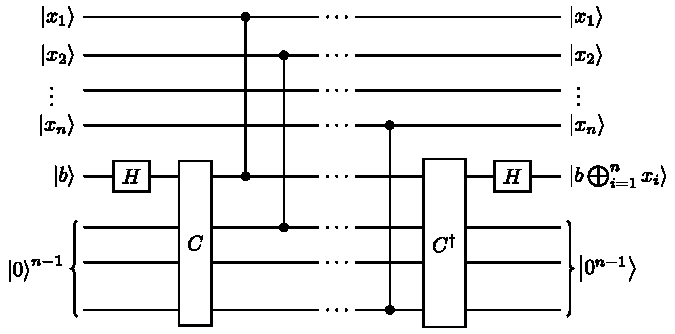
\includegraphics[width=\linewidth,height=0.78\textheight,keepaspectratio]{ccc2025-3-svg-05.pdf}\par



To see that this circuit exactly computes parity note that after the first Hadamard gate is applied the ancilla bits are in the state $\frac{\left|0\right\rangle+(-1)^{b}\left|1\right\rangle}{\sqrt{2}}\left|0^{n-1}\right\rangle$ and after applying $C$ we have $\frac{\left|0^{n}\right\rangle+(-1)^{b}\left|1^{n}\right\rangle}{\sqrt{2}}$. After the $\mathsf{CZ}$ gates are applied we are left with the state $\frac{\left|0^{n}\right\rangle+(-1)^{b+\sum_{i=1}^{n}x_{i}}\left|1^{n}\right\rangle}{\sqrt{2}}$. After applying $C^{{\dagger}}$ we are left with $\frac{\left|0\right\rangle+(-1)^{b+\sum_{i=1}^{n}x_{i}}\left|1\right\rangle}{\sqrt{2}}\left|0^{n-1}\right\rangle$, so the final Hadamard gate leaves the output qubit and the ancilla qubits in the state $\left|b\bigoplus_{i=1}^{n}x_{i}\right\rangle\left|0^{n-1}\right\rangle$.
$\blacktriangleleft$
It should be noted that when our circuit $C$ has property $(1)$ it is in some sense stronger than the guarantee $C\left|0^{n}\right\rangle=\frac{\left|0^{n}\right\rangle+\left|1^{n}\right\rangle}{2}$. In the case of the latter it seems that an $\mathsf{OR}$ gate is required to compute parity with $C$ and $C^{{\dagger}}$, which Proposition 28 shows is not necessary when $C(\alpha\left|0\right\rangle+\beta\left|1\right\rangle)\left|0^{n-1}\right\rangle=\alpha\left|0^{n}\right\rangle+\beta\left|1^{n}\right\rangle$ for all one-qubit states $\alpha\left|0\right\rangle+\beta\left|1\right\rangle$.\par




To see that (2) $\implies$ (1) note that\par


\[\begin{gathered}
\mathsf{F}_{n}\left|+\right\rangle\left|0^{n}\right\rangle=\frac{\left|0^{n+1}\right\rangle+\left|1^{n+1}\right\rangle}{\sqrt{2}}
\end{gathered}\]


Observe that if given access to some circuit $C$ (and $C^{{\dagger}}$) which satisfies the weaker condition of preparing an exact $n$-nekomata, i.e.,\par


\[\begin{gathered}
\displaystyle C\left|0^{m}\right\rangle=\frac{\left|0^{n}\right\rangle\left|\psi_{0}\right\rangle+\left|1^{n}\right\rangle\left|\psi_{1}\right\rangle}{\sqrt{2}}
\end{gathered}\]


one can construct a constant-depth ${\mathsf{QAC}}$ circuit which exactly computes Parity:\par



\par\noindent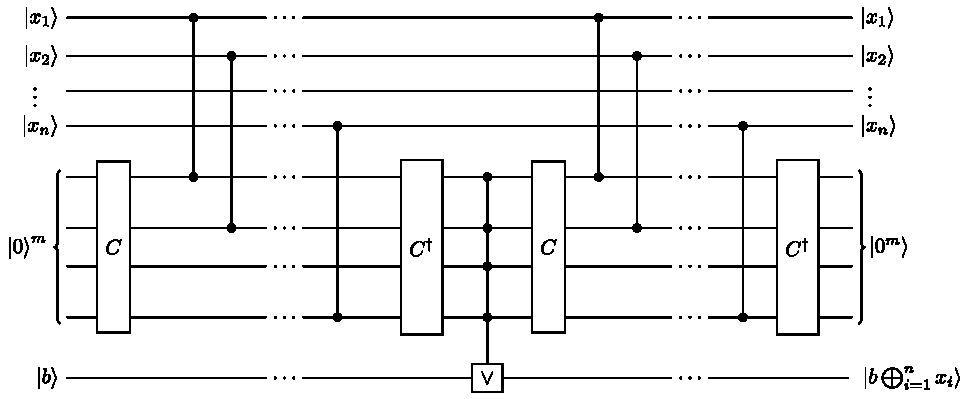
\includegraphics[width=\linewidth,height=0.78\textheight,keepaspectratio]{ccc2025-3-svg-06.pdf}\par

Figure 3: Computing $\mathsf{P}_{n}$ with a circuit $C$ which prepares an exact $n$-nekomata and its inverse $C^{{\dagger}}$.



Note that in the below circuit after the first layer of $\mathsf{CZ}$ gates are applied the state on the ancilla qubits is $\frac{\left|0^{n}\right\rangle\left|\psi_{0}\right\rangle+(-1)^{|x|}\left|1^{n}\right\rangle\left|\psi_{1}\right\rangle}{\sqrt{2}}$. When $|x|$ is even, nothing has happened, so $C^{{\dagger}}$ will return the state on these registers to $\left|0^{m}\right\rangle$ and the $\lor$-gate will not change the final register. When $|x|$ is odd $\frac{\left|0^{n}\right\rangle\left|\psi_{0}\right\rangle+(-1)^{|x|}\left|1^{n}\right\rangle\left|\psi_{1}\right\rangle}{\sqrt{2}}$ is orthogonal to $C\left|0^{m}\right\rangle$, so after applying $C^{{\dagger}}$ the resulting state is orthogonal to $\left|0^{m}\right\rangle$ which will always trigger the $\lor$-gate. The second half of the circuit uncomputes returning the ancillary registers to $\left|0^{m}\right\rangle$. Thus, the final register is always left in the state $\left|b\bigoplus_{i=1}^{n}x_{i}\right\rangle$ - thus, (up to an $X$ gate) this circuit exactly computes parity.\par




Finally, we prove Lemma 16 and in particular that the below circuit approximates $\mathsf{P}_{n}$ when $C$ is replaced with any $U$ which produces an $\epsilon$-approximate $n$-nekomata when applied to the all zeros state.\par





\par\medskip\noindent\textbf{Proof of Lemma 16.}\par




Let $U$ be a unitary on $m$ qubits such that $U\left|0^{m}\right\rangle=\left|\psi\right\rangle$ is an $\epsilon$-approximate $n$-nekomata and let $\left|\nu\right\rangle=\frac{\left|0^{n}\right\rangle\left|\psi_{0}\right\rangle+\left|1^{n}\right\rangle\left|\psi_{1}\right\rangle}{\sqrt{2}}$ be the $n$-nekomata on $m$ qubits which maximizes $|\left\langle\nu\middle|\psi\right\rangle|^{2}$. We can write $\left|\psi\right\rangle=\sqrt{1-\epsilon}\left|\nu\right\rangle+\sqrt{\epsilon}\left|\nu^{\perp}\right\rangle$ for some $\left|\nu^{\perp}\right\rangle$ which is orthogonal to $\left|\nu\right\rangle$. In the circuit shown in Figure 3 observe that after the first layer of $\mathsf{CZ}$ gates are applied the state on the ancilla registers is\par


\[\begin{gathered}
\displaystyle\left|\psi_{-}\right\rangle \displaystyle=\sqrt{1-\epsilon}\frac{\left|0^{n}\right\rangle\left|\psi_{0}\right\rangle+(-1)^{|x|}\left|1^{n}\right\rangle\left|\psi_{1}\right\rangle}{\sqrt{2}}+\sqrt{\epsilon}\left|\nu_{-}^{\perp}\right\rangle
\end{gathered}\]


For some $\left|\nu^{\perp}_{-}\right\rangle$. Observe that when $|x|$ is even then $|\left\langle\psi_{-}\middle|\psi\right\rangle|^{2}\geq 1-2\epsilon$ and when $|x|$ is odd then $|\left\langle\psi_{-}\middle|\psi\right\rangle|^{2}=O(\epsilon)$. In the former case $C^{{\dagger}}\left|\psi_{-}\right\rangle$ will have fidelity at least $1-O(\epsilon)$ with $\left|0^{m}\right\rangle$, so after uncomputation we are left with $\left|x,0^{m}\right\rangle\left|\omega_{b}\right\rangle$ where $|\left\langle b\middle|\omega_{b}\right\rangle|^{2}\geq 1-O(\epsilon)$. Similarly, when $|x|$ is odd $C^{{\dagger}}\left|\psi_{-}\right\rangle$ has fidelity at most $O(\epsilon)$ with $\left|0^{m}\right\rangle$ and after uncomputation we are left with $\left|x,0^{m}\right\rangle\left|\omega_{b}\right\rangle$ where $|\left\langle b\middle|\omega_{b}\right\rangle|^{2}\leq O(\epsilon)$. Thus, on any input $\left|x,b\right\rangle$ the state produced by this circuit has fidelity at least $1-O(\epsilon)$ with $F_{n}\left|x,b\right\rangle$ - equivalently, the $\ell_{2}$-distance is at most $O(\epsilon)$ meaning that the unitary implemented by this circuit, $V$, satisfies $\|V-\mathsf{P}_{n}\|_{\mathrm{op}}=O(\epsilon)$. Thus, (1) $\implies$ (3).\par




To see that (3) $\implies$ (2) suppose that the unitary $U$ satisfies $\|U-\mathsf{P}_{n}\|_{\mathrm{op}}\leq\epsilon$. Then,\par


\[\begin{gathered}
\displaystyle\|H^{\otimes(n+1)}UH^{\otimes(n+1)}-\mathsf{F}_{n}\|_{\mathrm{op}} \displaystyle=\|H^{\otimes(n+1)}(U-\mathsf{P}_{n})H^{\otimes(n+1)}\|_{\mathrm{op}}\leq\|U-\mathsf{P}_{n}\|_{\mathrm{op}}\leq\epsilon
\end{gathered}\]


For (2) $\implies$ (1) let $\left|\psi\right\rangle=\mathsf{F}_{n}\left|+\right\rangle\left|0^{n}\right\rangle=\frac{\left|0^{n}\right\rangle+\left|1^{n}\right\rangle}{\sqrt{2}}$ and $\left|\phi\right\rangle=U\left|+\right\rangle\left|0^{n}\right\rangle$. Note that if $\|U-\mathsf{F}_{n}\|_{\mathrm{op}}\leq\epsilon$ then\par


\[\begin{gathered}
\displaystyle\|\left|\phi\right\rangle-\left|\psi\right\rangle\|_{2}\leq\|\left|+\right\rangle\left|0^{n}\right\rangle\|_{2}\|U-\mathsf{F}_{n}\|_{\mathrm{op}}\leq\epsilon
\end{gathered}\]


So,\par


\[\begin{gathered}
\displaystyle\|\left|\phi\right\rangle-\left|\psi\right\rangle\|_{2} \displaystyle=\sqrt{2-\left\langle\psi\middle|\phi\right\rangle-\left\langle\phi\middle|\psi\right\rangle}\leq\epsilon\implies|\left\langle\psi\middle|\phi\right\rangle|^{2}\geq 1-\epsilon^{2}-\epsilon^{4}/4
\end{gathered}\]


Thus, $\left|\phi\right\rangle$ is an $O(\epsilon)$-approximate nekomata.
$\blacktriangleleft$\par





\par\medskip\noindent\textbf{Proof.}\par




Proof of Lemma 29
This can be seen via a direct computation:\par


\[\begin{gathered}
\displaystyle\mathsf{F}_{n,p}Q^{\otimes{n+1}}\left|b\right\rangle\left|x\right\rangle \displaystyle=\mathsf{F}_{n,p}\bigg{(}\frac{1}{\sqrt{p}}\sum_{j=0}^{p-1}\omega^{bj}\left|j\right\rangle\bigg{)}\otimes\bigg{(}\frac{1}{\sqrt{p^{n}}}\sum_{y\in\mathbb{F}_{p}^{n}}\omega^{\langle x,y\rangle}\left|y\right\rangle\bigg{)}
\end{gathered}\]


Here $\langle x,y\rangle$ denotes the inner product over vectors in $\mathbb{F}_{p}^{n}$: $\langle x,y\rangle=\sum_{j=1}^{p}x_{j}y_{j}\mod{p}$. For $y\in\mathbb{F}_{p}^{n}$ and $j\in\mathbb{F}_{p}$ we will use $y^{(j)}$ to denote the string obtained by adding $j$ to every entry of $y$, i.e., $F_{p}\left|j\right\rangle\left|y\right\rangle=\left|j\right\rangle\left|y^{(j)}\right\rangle$. Now we can see that\par


\[\begin{gathered}
\displaystyle\bigg{(}\frac{1}{\sqrt{p}}\sum_{j=0}^{p-1}\omega^{bj}\left|j\right\rangle\bigg{)}\otimes\bigg{(}\frac{1}{\sqrt{p^{n}}}\sum_{y\in\mathbb{F}_{p}^{n}}\omega^{\langle x,y\rangle}\left|y\right\rangle\bigg{)}=\frac{1}{\sqrt{p^{n+1}}}\sum_{y\in\mathbb{F}_{p}^{n}}\sum_{j=0}^{p-1}\omega^{bj+\langle
x,y\rangle}\left|j\right\rangle\left|y\right\rangle
\end{gathered}\]


So,\par


\[\begin{gathered}
\displaystyle\mathsf{F}_{n,p}\frac{1}{\sqrt{p^{n+1}}}\sum_{y\in\mathbb{F}_{p}^{n}}\sum_{j=0}^{p-1}\omega^{bj+\langle x,y\rangle}\left|j\right\rangle\left|y\right\rangle \displaystyle=\frac{1}{\sqrt{p^{n+1}}}\sum_{y\in\mathbb{F}_{p}^{n}}\sum_{j=0}^{p-1}\omega^{bj+\langle x,y\rangle}\left|j\right\rangle\left|y^{(j)}\right\rangle
\end{gathered}\]


After rearranging we have\par


\[\begin{gathered}
\displaystyle\frac{1}{\sqrt{p^{n+1}}}\sum_{y\in\mathbb{F}_{p}^{n}}\sum_{j=0}^{p-1}\omega^{bj+\langle x,y\rangle}\left|j\right\rangle\left|y^{(j)}\right\rangle \displaystyle=\frac{1}{\sqrt{p^{n+1}}}\sum_{y\in\mathbb{F}_{p}^{n}}\sum_{j=0}^{p-1}\omega^{bj+\langle x,y^{(-j)}\rangle}\left|j\right\rangle\left|y\right\rangle \\
\displaystyle=\frac{1}{\sqrt{p^{n+1}}}\sum_{y\in\mathbb{F}_{p}^{n}}\sum_{j=0}^{p-1}\omega^{bj+\langle x,y\rangle-j|x|}\left|j\right\rangle\left|y\right\rangle \\
\displaystyle=\frac{1}{\sqrt{p^{n+1}}}\sum_{y\in\mathbb{F}_{p}^{n}}\sum_{j=0}^{p-1}\omega^{\langle x,y\rangle}\omega^{j(b-|x|)}\left|j\right\rangle\left|y\right\rangle \\
\displaystyle=Q^{\otimes(n+1)}\mathsf{M}_{n,p}\left|b\right\rangle\left|x\right\rangle
\end{gathered}\]


Thus, $\mathsf{M}_{n,p}=(Q_{p}^{\dagger})^{\otimes{n+1}}\mathsf{F}_{n,p}Q_{p}^{\otimes{n+1}}$ as claimed.
$\blacktriangleleft$\par




\par




\end{document}
